\documentclass[aspectratio=169,xcolor=dvipsnames]{beamer}
\usetheme{SimplePlus}

% Math
\usepackage{nicefrac}

% Tipography stuff
\usepackage{booktabs} % Allows the use of \toprule, \midrule and \bottomrule in tables
\usepackage[english]{babel}
\usepackage{microtype}
\usepackage{pdfpages}
\usepackage{fontawesome5}
\usepackage{soul}
\usepackage{euler}

% Bibliography
\usepackage[giveninits,style=authoryear-comp,backend=biber]{biblatex}
\addbibresource{../fracbiblio.bib}
\newcommand\unnumbered{\setbeamertemplate{footline}{}\addtocounter{framenumber}{-1}}
\renewcommand*{\bibfont}{\normalfont\small}

% Figures
\usepackage{tikz,pgfplots}
\usetikzlibrary{calc,arrows}
\usepackage{subfig}
\usepackage{graphicx} % Allows including images

% Links
\usepackage{hyperref}
\hypersetup{colorlinks,linkcolor=,urlcolor=MidnightBlue}

% Code
\usepackage{minted}


\author{Fabio Durastante}
\title{An introduction to fractional calculus}
\subtitle{Fundamental ideas and numerics}
\institute{Università di Pisa\\\href{mailto:fabio.durastante@unipi.it}{\faEnvelope\;fabio.durastante@unipi.it}\\\href{https://fdurastante.github.io}{\faFirefox\;fdurastante.github.io}}
\date{May 2, 2022}

\newcommand{\de}{{\rm d}}


\begin{document}

\begin{frame}[t,plain]
\titlepage
\vspace{-4em}
\includegraphics[width=2cm]{frame.png}
\end{frame}

\begin{frame}{The original idea}
The \alert{concept of differentiation and integration to noninteger order} goes as far back as the concept we are used to work with. Leibniz mentions it in a letter to L'H\^{o}spital in 1695:\vspace{0.5em}

\begin{columns}
\begin{column}{0.7\columnwidth}
\begin{quote}
\small ``John Bernoulli seems to have told you of my having mentioned to him a
marvelous analogy which makes it possible to
say in a way that successive differentials are
in geometric progression. \textbf{One can ask what
would be a differential having as its exponent
a fraction}. You see that the result can be expressed
by an infinite series. Although this
seems removed from Geometry, which does
not yet know of such fractional exponents, \textbf{it
appears that one day these paradoxes will
yield useful consequences, since there is hardly
a paradox without utility}. Thoughts that
mattered little in themselves may give occasion
to more beautiful ones.''
\end{quote}
\end{column}
\begin{column}{0.25\columnwidth}
\centering\footnotesize
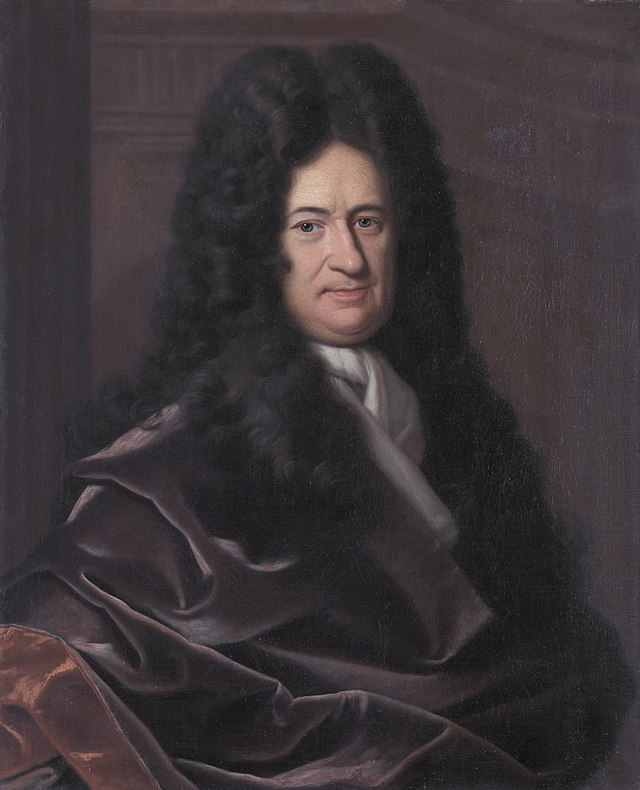
\includegraphics[width=\columnwidth]{Leibniz.jpg}

(Leibniz, 1646-1716)
\end{column}
\end{columns}
\end{frame}

\begin{frame}{Who cares?}
Derivatives of non integer order help
\begin{itemize}
	\item modeling of \emph{viscoelastic} phenomena, \emph{e.g.}, \parencite{MULLER20112938,BagleyTorvik}
	\item restate fundamental model from physics [gravity~\parencite{Giusti2020}, Schr\"odinger~\parencite{PhysRevE.66.056108}, waves~\parencite{LuchkoWave}, \ldots],
	\item modeling of heterogeneous cardiac tissues~\parencite{Cusimano2015},
	\item describing phenomena with \emph{memory} and \emph{non locality} aspects, \emph{e.g.}, \parencite{Riascos2014,BenziDurastante}\\
	\begin{center}
		\vdots
	\end{center}
\end{itemize}
This is a \textbf{booming topic}, and many new applications frequently arise.
\end{frame}

\section{Fractional integrals}

\begin{frame}{Fractional integrals}

\begin{columns}
\begin{column}{0.58\columnwidth}
\begin{alertblock}{Euler $\Gamma$-function}
The \textbf{$\Gamma$ function} $\Gamma(z)$ is defined for complex numbers with a
positive real part via the convergent improper integral:
\[
\Gamma(z) = \int_{0}^{+\infty} x^{z-1} e^{-x}\,{\rm d}x, \qquad \Re(z) > 0,
\]
and then extended by \textbf{analyitic continuation} to a \emph{meromorphic} function that is holomorphic in the whole complex plane except zero and the negative integers, where the function has simple poles.
\end{alertblock}
\end{column}
\begin{column}{0.4\columnwidth}
\centering

% This file was created by matlab2tikz.
%
%The latest updates can be retrieved from
%  http://www.mathworks.com/matlabcentral/fileexchange/22022-matlab2tikz-matlab2tikz
%where you can also make suggestions and rate matlab2tikz.
%
\definecolor{mycolor1}{rgb}{0.00000,0.44700,0.74100}%
%
\begin{tikzpicture}

\begin{axis}[%
width=0.7\columnwidth,
height=0.7\columnwidth,
at={(0.772in,0.481in)},
scale only axis,
unbounded coords=jump,
xmin=-5,
xmax=5,
ymin=-7,
ymax=7,
axis background/.style={fill=white}
]
\addplot [color=mycolor1, line width=2.0pt, forget plot]
  table[row sep=crcr]{%
-5	nan\\
-4.99	-0.847804719847104\\
-4.98	-0.431397805424746\\
-4.97	-0.292774913224111\\
-4.96	-0.22360295118331\\
-4.95	-0.182215504271632\\
-4.94	-0.154723946205723\\
-4.93	-0.135176170251616\\
-4.92	-0.120596272449079\\
-4.91	-0.10933111318748\\
-4.9	-0.100388942322004\\
-4.89	-0.0931387747028055\\
-4.88	-0.0871600784109484\\
-4.87	-0.0821618381248587\\
-4.86	-0.0779363060877115\\
-4.85	-0.0743312531651324\\
-4.84	-0.0712326262412292\\
-4.83	-0.068553327028887\\
-4.82	-0.0662257317845876\\
-4.81	-0.0641965737417148\\
-4.8	-0.0624233613547595\\
-4.79	-0.0608718204635276\\
-4.78	-0.0595140346331588\\
-4.77	-0.0583270712329557\\
-4.76	-0.0572919516345775\\
-4.75	-0.0563928692339824\\
-4.74	-0.0556165886369832\\
-4.73	-0.054951979105972\\
-4.72	-0.0543896487731796\\
-4.71	-0.0539216553734633\\
-4.7	-0.0535412757239197\\
-4.69	-0.0532428207733565\\
-4.68	-0.0530214863490228\\
-4.67	-0.0528732321324988\\
-4.66	-0.0527946831661337\\
-4.65	-0.0527830495075564\\
-4.64	-0.0528360606387437\\
-4.63	-0.0529519119866322\\
-4.62	-0.0531292214873842\\
-4.61	-0.053366994571513\\
-4.6	-0.0536645962950791\\
-4.59	-0.0540217296172827\\
-4.58	-0.054438419044932\\
-4.57	-0.0549149990429337\\
-4.56	-0.0554521067573634\\
-4.55	-0.0560506787217079\\
-4.54	-0.0567119513237315\\
-4.53	-0.0574374649050467\\
-4.52	-0.0582290714519893\\
-4.51	-0.0590889459182965\\
-4.5	-0.0600196013005042\\
-4.49	-0.0610239076688607\\
-4.48	-0.0621051154428169\\
-4.47	-0.0632668832938414\\
-4.46	-0.0645133111627579\\
-4.45	-0.0658489789978184\\
-4.44	-0.0672789919577612\\
-4.43	-0.0688090329865504\\
-4.42	-0.0704454238599533\\
-4.41	-0.0721951960367966\\
-4.4	-0.0740661729300365\\
-4.39	-0.0760670655578381\\
-4.38	-0.0782075839596178\\
-4.37	-0.0804985672883205\\
-4.36	-0.0829521361465728\\
-4.35	-0.0855818715581942\\
-4.34	-0.088403026007289\\
-4.33	-0.0914327733007335\\
-4.32	-0.0946905057048111\\
-4.31	-0.0981981889930105\\
-4.3	-0.101980788883433\\
-4.29	-0.106066786066908\\
-4.28	-0.110488801945592\\
-4.27	-0.115284363759578\\
-4.26	-0.120496846606347\\
-4.25	-0.126176641862679\\
-4.24	-0.132382618024806\\
-4.23	-0.13918396294746\\
-4.22	-0.14666252882175\\
-4.21	-0.154915847459068\\
-4.2	-0.164061050477614\\
-4.19	-0.174240027768013\\
-4.18	-0.185626305784188\\
-4.17	-0.198434353818002\\
-4.16	-0.212932380497728\\
-4.15	-0.229460249280949\\
-4.14	-0.248455072440962\\
-4.13	-0.270488618124792\\
-4.12	-0.296323421449111\\
-4.11	-0.326999502215204\\
-4.1	-0.363973113892433\\
-4.09	-0.409347992656189\\
-4.08	-0.466280044056746\\
-4.07	-0.539728904987631\\
-4.06	-0.637961068853317\\
-4.05	-0.775856762483229\\
-4.04	-0.983177140443137\\
-4.03	-1.32936587081244\\
-4.02	-2.02275548279152\\
-4.01	-4.10501180946578\\
-4	nan\\
-3.99	4.23054555203705\\
-3.98	2.14836107101519\\
-3.97	1.45509131872383\\
-3.96	1.10907063786922\\
-3.95	0.901966746144579\\
-3.94	0.764336294256265\\
-3.93	0.666418519340466\\
-3.92	0.593333660449468\\
-3.91	0.536815765750525\\
-3.9	0.491905817377817\\
-3.89	0.455448608296719\\
-3.88	0.425341182645428\\
-3.87	0.400128151668062\\
-3.86	0.378770447586278\\
-3.85	0.360506577850893\\
-3.84	0.344765911007549\\
-3.83	0.331112569549524\\
-3.82	0.319208027201712\\
-3.81	0.308785519697648\\
-3.8	0.299632134502846\\
-3.79	0.291576020020297\\
-3.78	0.284477085546499\\
-3.77	0.278220129781199\\
-3.76	0.272709689780589\\
-3.75	0.267866128861417\\
-3.74	0.263622630139301\\
-3.73	0.259922861171247\\
-3.72	0.256719142209408\\
-3.71	0.253970996809012\\
-3.7	0.251643995902423\\
-3.69	0.249708829427042\\
-3.68	0.248140556113427\\
-3.67	0.246917994058769\\
-3.66	0.246023223554183\\
-3.65	0.245441180210137\\
-3.64	0.245159321363771\\
-3.63	0.245167352498107\\
-3.62	0.245457003271715\\
-3.61	0.246021844974675\\
-3.6	0.246857142957364\\
-3.59	0.247959738943327\\
-3.58	0.249327959225788\\
-3.57	0.250961545626207\\
-3.56	0.252861606813577\\
-3.55	0.255030588183771\\
-3.54	0.257472259009741\\
-3.53	0.260191716019861\\
-3.52	0.263195402962992\\
-3.51	0.266491146091517\\
-3.5	0.270088205852269\\
-3.49	0.273997345433184\\
-3.48	0.27823091718382\\
-3.47	0.282802968323471\\
-3.46	0.2877293677859\\
-3.45	0.293027956540292\\
-3.44	0.29871872429246\\
-3.43	0.304824016130418\\
-3.42	0.311368773460994\\
-3.41	0.318380814522273\\
-3.4	0.32589116089216\\
-3.39	0.333934417798909\\
-3.38	0.342549217743126\\
-3.37	0.351778739049961\\
-3.36	0.361671313599058\\
-3.35	0.372281141278144\\
-3.34	0.383669132871634\\
-3.33	0.395903908392176\\
-3.32	0.409062984644784\\
-3.31	0.423234194559876\\
-3.3	0.438517392198763\\
-3.29	0.455026512227037\\
-3.28	0.472892072327136\\
-3.27	0.492264233253396\\
-3.26	0.513316566543036\\
-3.25	0.536250727916385\\
-3.24	0.561302300425176\\
-3.23	0.588748163267756\\
-3.22	0.618915871627785\\
-3.21	0.652195717802675\\
-3.2	0.689056412005979\\
-3.19	0.730065716347971\\
-3.18	0.775917958177905\\
-3.17	0.827471255421066\\
-3.16	0.885798702870549\\
-3.15	0.952260034515942\\
-3.14	1.02860399990558\\
-3.13	1.11711799285539\\
-3.12	1.22085249637034\\
-3.11	1.34396795410449\\
-3.1	1.49228976695897\\
-3.09	1.67423328996381\\
-3.08	1.90242257975152\\
-3.07	2.19669664329966\\
-3.06	2.59012193954448\\
-3.05	3.14221988805708\\
-3.04	3.97203564739027\\
-3.03	5.35734445937414\\
-3.02	8.13147704082174\\
-3.01	nan\\
-3	nan\\
-2.99	nan\\
-2.98	-8.55047706264044\\
-2.97	-5.77671253533368\\
-2.96	-4.39191972596211\\
-2.95	-3.56276864727109\\
-2.94	-3.01148499936968\\
-2.93	-2.61902478100805\\
-2.92	-2.32586794896191\\
-2.91	-2.09894964408455\\
-2.9	-1.91843268777349\\
-2.89	-1.77169508627424\\
-2.88	-1.65032378866426\\
-2.87	-1.5484959469554\\
-2.86	-1.46205392768303\\
-2.85	-1.38795032472594\\
-2.84	-1.32390109826899\\
-2.83	-1.26816114137468\\
-2.82	-1.21937466391054\\
-2.81	-1.17647283004804\\
-2.8	-1.13860211111081\\
-2.79	-1.10507311587693\\
-2.78	-1.07532338336576\\
-2.77	-1.04888988927512\\
-2.76	-1.02538843357501\\
-2.75	-1.00449798323031\\
-2.74	-0.985948636720984\\
-2.73	-0.969512272168753\\
-2.72	-0.954995209018997\\
-2.71	-0.942232398161435\\
-2.7	-0.931082784838964\\
-2.69	-0.921425580585784\\
-2.68	-0.91315724649741\\
-2.67	-0.906189038195683\\
-2.66	-0.90044499820831\\
-2.65	-0.895860307767001\\
-2.64	-0.892379929764126\\
-2.63	-0.889957489568128\\
-2.62	-0.888554351843609\\
-2.61	-0.888138860358577\\
-2.6	-0.88868571464651\\
-2.59	-0.890175462806545\\
-2.58	-0.892594094028322\\
-2.57	-0.89593271788556\\
-2.56	-0.900187320256334\\
-2.55	-0.905358588052387\\
-2.54	-0.911451796894484\\
-2.53	-0.918476757550111\\
-2.52	-0.92644781842973\\
-2.51	-0.935383922781226\\
-2.5	-0.945308720482942\\
-2.49	-0.956250735561814\\
-2.48	-0.968243591799693\\
-2.47	-0.981326300082443\\
-2.46	-0.995543612539215\\
-2.45	-1.01094645006401\\
-2.44	-1.02759241156606\\
-2.43	-1.04554637532733\\
-2.42	-1.0648812052366\\
-2.41	-1.08567857752095\\
-2.4	-1.10802994703335\\
-2.39	-1.1320376763383\\
-2.38	-1.15781635597177\\
-2.37	-1.18549435059837\\
-2.36	-1.21521561369283\\
-2.35	-1.24714182328178\\
-2.34	-1.28145490379126\\
-2.33	-1.31836001494595\\
-2.32	-1.35808910902068\\
-2.31	-1.40090518399319\\
-2.3	-1.44710739425592\\
-2.29	-1.49703722522695\\
-2.28	-1.55108599723301\\
-2.27	-1.6097040427386\\
-2.26	-1.6734120069303\\
-2.25	-1.74281486572825\\
-2.24	-1.81861945337757\\
-2.23	-1.90165656735485\\
-2.22	-1.99290910664146\\
-2.21	-2.09354825414659\\
-2.2	-2.20498051841913\\
-2.19	-2.32890963515003\\
-2.18	-2.46741910700573\\
-2.17	-2.62308387968478\\
-2.16	-2.79912390107094\\
-2.15	-2.99961910872522\\
-2.14	-3.22981655970352\\
-2.13	-3.49657931763737\\
-2.12	-3.80905978867545\\
-2.11	-4.17974033726498\\
-2.1	-4.62609827757281\\
-2.09	-5.17338086598819\\
-2.08	-5.85946154563469\\
-2.07	-6.74385869492999\\
-2.06	-7.92577313500613\\
-2.05	-9.58377065857409\\
-2.04	nan\\
-2.03	nan\\
-2.02	nan\\
-2.01	nan\\
-2	nan\\
-1.99	nan\\
-1.98	nan\\
-1.97	nan\\
-1.96	nan\\
-1.95	nan\\
-1.94	8.85376589814687\\
-1.93	7.67374260835358\\
-1.92	6.79153441096879\\
-1.91	6.10794346428605\\
-1.9	5.56345479454311\\
-1.89	5.12019879933256\\
-1.88	4.75293251135307\\
-1.87	4.444183367762\\
-1.86	4.18147423317347\\
-1.85	3.95565842546892\\
-1.84	3.75987911908393\\
-1.83	3.58889603009034\\
-1.82	3.43863655222772\\
-1.81	3.30588865243499\\
-1.8	3.18808591111028\\
-1.79	3.08315399329662\\
-1.78	2.98939900575683\\
-1.77	2.90542499329208\\
-1.76	2.83007207666704\\
-1.75	2.76236945388336\\
-1.74	2.7014992646155\\
-1.73	2.6467685030207\\
-1.72	2.59758696853167\\
-1.71	2.55344979901749\\
-1.7	2.5139235190652\\
-1.69	2.47863481177576\\
-1.68	2.44726142061306\\
-1.67	2.41952473198247\\
-1.66	2.3951836952341\\
-1.65	2.37402981558255\\
-1.64	2.35588301457729\\
-1.63	2.34058819756418\\
-1.62	2.32801240183026\\
-1.61	2.31804242553589\\
-1.6	2.31058285808093\\
-1.59	2.30555444866895\\
-1.58	2.30289276259307\\
-1.57	2.30254708496589\\
-1.56	2.30447953985622\\
-1.55	2.30866439953359\\
-1.54	2.31508756411199\\
-1.53	2.32374619660178\\
-1.52	2.33464850244292\\
-1.51	2.34781364618088\\
-1.5	2.36327180120735\\
-1.49	2.38106433154892\\
-1.48	2.40124410766324\\
-1.47	2.42387596120364\\
-1.46	2.44903728684647\\
-1.45	2.47681880265682\\
-1.44	2.50732548422119\\
-1.43	2.54067769204542\\
-1.42	2.57701251667257\\
-1.41	2.61648537182549\\
-1.4	2.65927187288003\\
-1.39	2.70557004644854\\
-1.38	2.7556029272128\\
-1.37	2.80962161091813\\
-1.36	2.86790884831509\\
-1.35	2.93078328471219\\
-1.34	2.99860447487154\\
-1.33	3.07177883482405\\
-1.32	3.15076673292799\\
-1.31	3.23609097502427\\
-1.3	3.32834700678861\\
-1.29	3.42821524576972\\
-1.28	3.53647607369126\\
-1.27	3.65402817701663\\
-1.26	3.78191113566247\\
-1.25	3.92133344788857\\
-1.24	4.07370757556576\\
-1.23	4.24069414520132\\
-1.22	4.42425821674405\\
-1.21	4.62674164166396\\
-1.2	4.85095714052209\\
-1.19	5.10031210097856\\
-1.18	5.37897365327249\\
-1.17	5.69209201891597\\
-1.16	6.04610762631322\\
-1.15	6.44918108375922\\
-1.14	6.91180743776554\\
-1.13	7.4477139465676\\
-1.12	8.07520675199195\\
-1.11	8.81925211162911\\
-1.1	9.7148063829029\\
-1.09	nan\\
-1.08	nan\\
-1.07	nan\\
-1.06	nan\\
-1.05	nan\\
-1.04	nan\\
-1.03	nan\\
-1.02	nan\\
-1.01	nan\\
-1	nan\\
-0.99	nan\\
-0.98	nan\\
-0.97	nan\\
-0.96	nan\\
-0.95	nan\\
-0.94	nan\\
-0.93	nan\\
-0.92	nan\\
-0.91	nan\\
-0.9	nan\\
-0.89	-9.6771757307385\\
-0.88	-8.93551312134378\\
-0.87	-8.31062289771493\\
-0.86	-7.77754207370267\\
-0.85	-7.31796808711749\\
-0.84	-6.91817757911443\\
-0.83	-6.56767973506532\\
-0.82	-6.25831852505446\\
-0.81	-5.98365846090733\\
-0.8	-5.7385546399985\\
-0.79	-5.51884564800096\\
-0.78	-5.32113023024716\\
-0.77	-5.14260223812698\\
-0.76	-4.98092685493398\\
-0.75	-4.83414654429588\\
-0.74	-4.70060872043097\\
-0.73	-4.57890951022581\\
-0.72	-4.46784958587447\\
-0.71	-4.36639915631991\\
-0.7	-4.27366998241085\\
-0.69	-4.18889283190104\\
-0.68	-4.11139918662994\\
-0.67	-4.04060630241073\\
-0.66	-3.97600493408861\\
-0.65	-3.91714919571121\\
-0.64	-3.86364814390676\\
-0.63	-3.81515876202961\\
-0.62	-3.77138009096501\\
-0.61	-3.73204830511278\\
-0.6	-3.69693257292948\\
-0.59	-3.66583157338363\\
-0.58	-3.63857056489705\\
-0.57	-3.61499892339645\\
-0.56	-3.59498808217569\\
-0.55	-3.57842981927706\\
-0.54	-3.56523484873246\\
-0.53	-3.55533168080072\\
-0.52	-3.54866572371324\\
-0.51	-3.54519860573312\\
-0.5	-3.54490770181103\\
-0.49	-3.54778585400789\\
-0.48	-3.55384127934159\\
-0.47	-3.56309766296935\\
-0.46	-3.57559443879584\\
-0.45	-3.59138726385239\\
-0.44	-3.61054869727851\\
-0.43	-3.63316909962495\\
-0.42	-3.65935777367504\\
-0.41	-3.68924437427394\\
-0.4	-3.72298062203204\\
-0.39	-3.76074236456347\\
-0.38	-3.80273203955367\\
-0.37	-3.84918160695784\\
-0.36	-3.90035603370852\\
-0.35	-3.95655743436146\\
-0.34	-4.01812999632787\\
-0.33	-4.08546585031599\\
-0.32	-4.15901208746494\\
-0.31	-4.23927917728179\\
-0.3	-4.32685110882519\\
-0.29	-4.42239766704294\\
-0.28	-4.52668937432481\\
-0.27	-4.64061578481113\\
-0.26	-4.76520803093471\\
-0.25	-4.90166680986071\\
-0.24	-5.05139739370154\\
-0.23	-5.21605379859762\\
-0.22	-5.39759502442775\\
-0.21	-5.59835738641339\\
-0.2	-5.82114856862651\\
-0.19	-6.06937140016447\\
-0.18	-6.34718891086156\\
-0.17	-6.65974766213169\\
-0.16	-7.01348484652334\\
-0.15	-7.41655824632309\\
-0.14	-7.87946047905274\\
-0.13	-8.41591675962139\\
-0.12	-9.04423156223099\\
-0.11	-9.78936984390828\\
-0.0999999999999996	nan\\
-0.0899999999999999	nan\\
-0.0800000000000001	nan\\
-0.0700000000000003	nan\\
-0.0599999999999996	nan\\
-0.0499999999999998	nan\\
-0.04	nan\\
-0.0300000000000002	nan\\
-0.0199999999999996	nan\\
-0.00999999999999979	nan\\
0	nan\\
0.00999999999999979	nan\\
0.0199999999999996	nan\\
0.0300000000000002	nan\\
0.04	nan\\
0.0499999999999998	nan\\
0.0599999999999996	nan\\
0.0700000000000003	nan\\
0.0800000000000001	nan\\
0.0899999999999999	nan\\
0.0999999999999996	9.51350769866877\\
0.11	8.61268640035726\\
0.12	7.86325154678252\\
0.13	7.23024192101199\\
0.14	6.6886861833843\\
0.15	6.22027287404986\\
0.16	5.81126916645612\\
0.17	5.45117418010421\\
0.18	5.13182119054466\\
0.19	4.84676335333493\\
0.2	4.5908437119988\\
0.21	4.35988806192076\\
0.22	4.15048157959278\\
0.23	3.95980372335777\\
0.24	3.78550440974983\\
0.25	3.62560990822191\\
0.26	3.47845045311892\\
0.27	3.34260394246484\\
0.28	3.21685170182962\\
0.29	3.10014340098713\\
0.3	2.99156898768759\\
0.31	2.89033605401172\\
0.32	2.79575144690836\\
0.33	2.70720622261519\\
0.34	2.62416325649848\\
0.35	2.54614697721229\\
0.36	2.47273481210032\\
0.37	2.40355002007865\\
0.38	2.33825565639831\\
0.39	2.2765494661188\\
0.4	2.21815954375769\\
0.41	2.16284062829634\\
0.42	2.11037092764029\\
0.43	2.06054938633598\\
0.44	2.01319332601839\\
0.45	1.96813640060238\\
0.46	1.92522681831553\\
0.47	1.88432579082439\\
0.48	1.84530617633088\\
0.49	1.80805128892389\\
0.5	1.77245385090552\\
0.51	1.73841506846386\\
0.52	1.70584381408397\\
0.53	1.67465590159559\\
0.54	1.64477344184609\\
0.55	1.61612426873358\\
0.56	1.58864142680255\\
0.57	1.56226271283873\\
0.58	1.53693026494352\\
0.59	1.51259019345232\\
0.6	1.48919224881282\\
0.61	1.46668952217975\\
0.62	1.44503817503039\\
0.63	1.4241971945744\\
0.64	1.40412817213507\\
0.65	1.38479510202651\\
0.66	1.36616419875147\\
0.67	1.34820373060428\\
0.68	1.33088386798878\\
0.69	1.31417654495735\\
0.7	1.29805533264756\\
0.71	1.28249532344245\\
0.72	1.26747302481095\\
0.73	1.252966261899\\
0.74	1.23895408804302\\
0.75	1.22541670246518\\
0.76	1.21233537448837\\
0.77	1.19969237367745\\
0.78	1.1874709053741\\
0.79	1.17565505114681\\
0.8	1.1642297137253\\
0.81	1.15318056603125\\
0.82	1.14249400395508\\
0.83	1.13215710256239\\
0.84	1.12215757544374\\
0.85	1.11248373694847\\
0.86	1.10312446706738\\
0.87	1.09406917875078\\
0.88	1.08530778746772\\
0.89	1.07683068282991\\
0.9	1.06862870211932\\
0.91	1.06069310557269\\
0.92	1.0530155532891\\
0.93	1.04558808363803\\
0.94	1.03840309305596\\
0.95	1.03145331712903\\
0.96	1.02473181286759\\
0.97	1.01823194208659\\
0.98	1.01194735581251\\
0.99	1.00587197964411\\
1	1\\
1.01	0.994325851191506\\
1.02	0.988844203263914\\
1.03	0.983549950553824\\
1.04	0.978438200914245\\
1.05	0.973504265562776\\
1.06	0.968743649511639\\
1.07	0.964152042541366\\
1.08	0.959725310682822\\
1.09	0.955459488174801\\
1.1	0.951350769866873\\
1.11	0.947395504039302\\
1.12	0.943590185613904\\
1.13	0.939931449731558\\
1.14	0.9364160656738\\
1.15	0.933040931107482\\
1.16	0.92980306663298\\
1.17	0.926699610617716\\
1.18	0.923727814298037\\
1.19	0.920885037133639\\
1.2	0.918168742399761\\
1.21	0.915576493003359\\
1.22	0.913105947510411\\
1.23	0.910754856372289\\
1.24	0.908521058339959\\
1.25	0.906402477055477\\
1.26	0.904397117810918\\
1.27	0.902503064465506\\
1.28	0.900718476512294\\
1.29	0.899041586286269\\
1.3	0.897470696306277\\
1.31	0.896004176743632\\
1.32	0.894640463010675\\
1.33	0.893378053463013\\
1.34	0.892215507209484\\
1.35	0.891151442024301\\
1.36	0.890184532356117\\
1.37	0.889313507429102\\
1.38	0.888537149431357\\
1.39	0.88785429178633\\
1.4	0.887263817503075\\
1.41	0.886764657601501\\
1.42	0.886355789608922\\
1.43	0.886036236124469\\
1.44	0.885805063448092\\
1.45	0.885661380271072\\
1.46	0.885604336425144\\
1.47	0.885633121687461\\
1.48	0.885746964638824\\
1.49	0.885945131572707\\
1.5	0.886226925452758\\
1.51	0.886591684916571\\
1.52	0.887038783323661\\
1.53	0.887567627845664\\
1.54	0.888177658596888\\
1.55	0.888868347803466\\
1.56	0.889639199009425\\
1.57	0.890489746318076\\
1.58	0.891419553667241\\
1.59	0.892428214136867\\
1.6	0.89351534928769\\
1.61	0.894680608529649\\
1.62	0.895923668518844\\
1.63	0.897244232581873\\
1.64	0.898642030166443\\
1.65	0.900116816317232\\
1.66	0.901668371175973\\
1.67	0.903296499504866\\
1.68	0.905001030232371\\
1.69	0.906781816020575\\
1.7	0.908638732853291\\
1.71	0.910571679644141\\
1.72	0.912580577863881\\
1.73	0.914665371186273\\
1.74	0.916826025151839\\
1.75	0.919062526848883\\
1.76	0.921374884611161\\
1.77	0.923763127731639\\
1.78	0.926227306191801\\
1.79	0.928767490405982\\
1.8	0.931383770980243\\
1.81	0.934076258485314\\
1.82	0.936845083243165\\
1.83	0.939690395126781\\
1.84	0.942612363372738\\
1.85	0.945611176406195\\
1.86	0.948687041677948\\
1.87	0.951840185513178\\
1.88	0.955070852971593\\
1.89	0.958379307718623\\
1.9	0.961765831907388\\
1.91	0.965230726071148\\
1.92	0.968774309025974\\
1.93	0.972396917783367\\
1.94	0.976098907472606\\
1.95	0.979880651272581\\
1.96	0.983742540352887\\
1.97	0.987684983823992\\
1.98	0.991708408696261\\
1.99	0.995813259847667\\
2	1\\
2.01	1.00426910970342\\
2.02	1.00862108732919\\
2.03	1.01305644907044\\
2.04	1.01757572895081\\
2.05	1.02217947884091\\
2.06	1.02686826848234\\
2.07	1.03164268551926\\
2.08	1.03650333553745\\
2.09	1.04145084211053\\
2.1	1.04648584685356\\
2.11	1.05160900948363\\
2.12	1.05682100788757\\
2.13	1.06212253819666\\
2.14	1.06751431486813\\
2.15	1.0729970707736\\
2.16	1.07857155729426\\
2.17	1.08423854442273\\
2.18	1.08999882087168\\
2.19	1.09585319418903\\
2.2	1.10180249087971\\
2.21	1.10784755653406\\
2.22	1.1139892559627\\
2.23	1.12022847333792\\
2.24	1.12656611234155\\
2.25	1.13300309631935\\
2.26	1.13954036844176\\
2.27	1.14617889187119\\
2.28	1.15291964993574\\
2.29	1.15976364630929\\
2.3	1.16671190519816\\
2.31	1.17376547153416\\
2.32	1.18092541117409\\
2.33	1.18819281110581\\
2.34	1.19556877966071\\
2.35	1.20305444673281\\
2.36	1.21065096400432\\
2.37	1.21835950517787\\
2.38	1.22618126621527\\
2.39	1.234117465583\\
2.4	1.24216934450431\\
2.41	1.25033816721812\\
2.42	1.25862522124467\\
2.43	1.26703181765799\\
2.44	1.27555929136525\\
2.45	1.28420900139305\\
2.46	1.29298233118071\\
2.47	1.30188068888057\\
2.48	1.31090550766546\\
2.49	1.32005824604333\\
2.5	1.32934038817914\\
2.51	1.33875344422402\\
2.52	1.34829895065196\\
2.53	1.35797847060387\\
2.54	1.36779359423921\\
2.55	1.37774593909537\\
2.56	1.3878371504547\\
2.57	1.39806890171938\\
2.58	1.40844289479424\\
2.59	1.41896086047762\\
2.6	1.4296245588603\\
2.61	1.44043577973274\\
2.62	1.45139634300053\\
2.63	1.46250809910845\\
2.64	1.47377292947297\\
2.65	1.48519274692343\\
2.66	1.49676949615212\\
2.67	1.50850515417313\\
2.68	1.52040173079038\\
2.69	1.53246126907477\\
2.7	1.54468584585059\\
2.71	1.55707757219148\\
2.72	1.56963859392588\\
2.73	1.58237109215225\\
2.74	1.5952772837642\\
2.75	1.60835942198555\\
2.76	1.62161979691564\\
2.77	1.635060736085\\
2.78	1.64868460502141\\
2.79	1.66249380782671\\
2.8	1.67649078776444\\
2.81	1.69067802785842\\
2.82	1.70505805150256\\
2.83	1.71963342308201\\
2.84	1.73440674860584\\
2.85	1.74938067635146\\
2.86	1.76455789752098\\
2.87	1.77994114690964\\
2.88	1.7955332035866\\
2.89	1.8113368915882\\
2.9	1.82735508062404\\
2.91	1.84359068679589\\
2.92	1.86004667332987\\
2.93	1.8767260513219\\
2.94	1.89363188049686\\
2.95	1.91076726998153\\
2.96	1.92813537909166\\
2.97	1.94573941813326\\
2.98	1.9635826492186\\
2.99	1.98166838709686\\
3	2\\
3.01	2.01858091050388\\
3.02	2.03741459640497\\
3.03	2.05650459161299\\
3.04	2.07585448705966\\
3.05	2.09546793162388\\
3.06	2.11534863307361\\
3.07	2.13550035902487\\
3.08	2.15592693791789\\
3.09	2.17663226001101\\
3.1	2.19762027839248\\
3.11	2.21889501001045\\
3.12	2.24046053672165\\
3.13	2.26232100635889\\
3.14	2.2844806338178\\
3.15	2.30694370216325\\
3.16	2.3297145637556\\
3.17	2.35279764139732\\
3.18	2.37619742950027\\
3.19	2.39991849527398\\
3.2	2.42396547993537\\
3.21	2.44834309994028\\
3.22	2.4730561482372\\
3.23	2.49810949554355\\
3.24	2.52350809164507\\
3.25	2.54925696671853\\
3.26	2.57536123267837\\
3.27	2.60182608454761\\
3.28	2.62865680185348\\
3.29	2.65585875004826\\
3.3	2.68343738195577\\
3.31	2.7113982392439\\
3.32	2.73974695392389\\
3.33	2.76848924987653\\
3.34	2.79763094440606\\
3.35	2.82717794982209\\
3.36	2.85713627505019\\
3.37	2.88751202727155\\
3.38	2.91831141359235\\
3.39	2.94954074274337\\
3.4	2.98120642681033\\
3.41	3.01331498299566\\
3.42	3.0458730354121\\
3.43	3.07888731690892\\
3.44	3.11236467093121\\
3.45	3.14631205341298\\
3.46	3.18073653470455\\
3.47	3.215645301535\\
3.48	3.25104565901034\\
3.49	3.2869450326479\\
3.5	3.32335097044784\\
3.51	3.36027114500229\\
3.52	3.39771335564295\\
3.53	3.43568553062778\\
3.54	3.47419572936758\\
3.55	3.5132521446932\\
3.56	3.55286310516404\\
3.57	3.59303707741881\\
3.58	3.63378266856914\\
3.59	3.67510862863703\\
3.6	3.71702385303679\\
3.61	3.75953738510244\\
3.62	3.80265841866138\\
3.63	3.84639630065523\\
3.64	3.89076053380864\\
3.65	3.9357607793471\\
3.66	3.98140685976463\\
3.67	4.02770876164225\\
3.68	4.07467663851823\\
3.69	4.12232081381113\\
3.7	4.1706517837966\\
3.71	4.21968022063892\\
3.72	4.26941697547839\\
3.73	4.31987308157565\\
3.74	4.37105975751391\\
3.75	4.42298841046025\\
3.76	4.47567063948718\\
3.77	4.52911823895545\\
3.78	4.5833432019595\\
3.79	4.63835772383651\\
3.8	4.69417420574043\\
3.81	4.75080525828216\\
3.82	4.80826370523722\\
3.83	4.86656258732209\\
3.84	4.92571516604058\\
3.85	4.98573492760166\\
3.86	5.04663558691001\\
3.87	5.10843109163067\\
3.88	5.1711356263294\\
3.89	5.23476361668989\\
3.9	5.29932973380971\\
3.91	5.36484889857605\\
3.92	5.43133628612322\\
3.93	5.49880733037316\\
3.94	5.56727772866075\\
3.95	5.63676344644552\\
3.96	5.70728072211131\\
3.97	5.7788460718558\\
3.98	5.85147629467142\\
3.99	5.9251884774196\\
4	6\\
4.01	6.07592854061667\\
4.02	6.152992081143\\
4.03	6.23120891258736\\
4.04	6.31059764066136\\
4.05	6.39117719145282\\
4.06	6.47296681720526\\
4.07	6.55598610220636\\
4.08	6.64025496878711\\
4.09	6.72579368343404\\
4.1	6.81262286301668\\
4.11	6.90076348113249\\
4.12	6.99023687457155\\
4.13	7.08106474990333\\
4.14	7.1732691901879\\
4.15	7.26687266181424\\
4.16	7.36189802146768\\
4.17	7.4583685232295\\
4.18	7.55630782581086\\
4.19	7.65573999992399\\
4.2	7.75668953579317\\
4.21	7.85918135080831\\
4.22	7.96324079732378\\
4.23	8.06889367060568\\
4.24	8.17616621693003\\
4.25	8.28508514183522\\
4.26	8.39567761853148\\
4.27	8.50797129647067\\
4.28	8.62199431007941\\
4.29	8.73777528765879\\
4.3	8.85534336045405\\
4.31	8.97472817189733\\
4.32	9.09595988702732\\
4.33	9.21906920208885\\
4.34	9.34408735431624\\
4.35	9.47104613190401\\
4.36	9.59997788416865\\
4.37	9.73091553190511\\
4.38	9.86389257794215\\
4.39	9.99894311790002\\
4.4	nan\\
4.41	nan\\
4.42	nan\\
4.43	nan\\
4.44	nan\\
4.45	nan\\
4.46	nan\\
4.47	nan\\
4.48	nan\\
4.49	nan\\
4.5	nan\\
4.51	nan\\
4.52	nan\\
4.53	nan\\
4.54	nan\\
4.55	nan\\
4.56	nan\\
4.57	nan\\
4.58	nan\\
4.59	nan\\
4.6	nan\\
4.61	nan\\
4.62	nan\\
4.63	nan\\
4.64	nan\\
4.65	nan\\
4.66	nan\\
4.67	nan\\
4.68	nan\\
4.69	nan\\
4.7	nan\\
4.71	nan\\
4.72	nan\\
4.73	nan\\
4.74	nan\\
4.75	nan\\
4.76	nan\\
4.77	nan\\
4.78	nan\\
4.79	nan\\
4.8	nan\\
4.81	nan\\
4.82	nan\\
4.83	nan\\
4.84	nan\\
4.85	nan\\
4.86	nan\\
4.87	nan\\
4.88	nan\\
4.89	nan\\
4.9	nan\\
4.91	nan\\
4.92	nan\\
4.93	nan\\
4.94	nan\\
4.95	nan\\
4.96	nan\\
4.97	nan\\
4.98	nan\\
4.99	nan\\
5	nan\\
};
\addplot [color=black, dashed, forget plot]
  table[row sep=crcr]{%
-4	-10\\
-4	10\\
};
\addplot [color=black, dashed, forget plot]
  table[row sep=crcr]{%
-3	-10\\
-3	10\\
};
\addplot [color=black, dashed, forget plot]
  table[row sep=crcr]{%
-2	-10\\
-2	10\\
};
\addplot [color=black, dashed, forget plot]
  table[row sep=crcr]{%
-1	-10\\
-1	10\\
};
\addplot [color=black, dashed, forget plot]
  table[row sep=crcr]{%
-4	-10\\
-4	10\\
};
\addplot [color=black, dashed, forget plot]
  table[row sep=crcr]{%
-3	-10\\
-3	10\\
};
\addplot [color=black, dashed, forget plot]
  table[row sep=crcr]{%
-2	-10\\
-2	10\\
};
\addplot [color=black, dashed, forget plot]
  table[row sep=crcr]{%
-1	-10\\
-1	10\\
};
\addplot [color=black, dashed, forget plot]
  table[row sep=crcr]{%
0	-10\\
0	10\\
};
\end{axis}
\end{tikzpicture}%

$\Gamma(z + 1) = z\, \Gamma(z)$

Bounded in: $S = \{z \in \mathbb{C} \,:\, \Re z \in [1,2)\}$
\end{column}
\end{columns}

\end{frame}

\begin{frame}[fragile]{A formula for repeated integration}

\begin{columns}
\begin{column}{0.65\columnwidth}
\begin{block}{Swapping Integrals}
If $G(x,t)$ is jointly continuous on $[c,b]\times[c,b]$:
\[
\int_{c}^{x} {\rm d}x_1 \int_{c}^{x_1} G(x_1,x_2) {\rm d}x_2 = \int_{c}^{x} {\rm d}x_2 \int_{x_2}^{x}G(x_1,x_2) {\rm d}x_1.
\]
\end{block}
\begin{alertblock}<2->{Fubini's Theorem}\small
Given $(X,\mathfrak{S}_X,\mu_x)$, $(Y,\mathfrak{S}_Y,\mu_y)$ measure spaces with $\sigma$-finite complete measures $\mu_x$, $\mu_y$ on the $\sigma$-algebras $\mathfrak{S}_X$, and $\mathfrak{S}_Y$. If the
function $f(x,y)$ is integrable on the product $X \times Y$ w.r.t. the product measure $\mu = \mu_x \times \mu_y$, then the following equality
holds true
\[ 
\int_{X \times Y} f(x,y)\,\textrm{d}\mu = \int_{Y} \textrm{d}\mu_y \int_X f(x,y) \textrm{d}\mu_x.
\]
\end{alertblock}
\end{column}
\begin{column}{0.35\columnwidth}
\begin{onlyenv}<2>
	\definecolor{cccccc}{rgb}{0.8,0.8,0.8}
	\definecolor{tttttt}{rgb}{0.2,0.2,0.2}
	\begin{tikzpicture}[line cap=round,line join=round,>=triangle 45,x=0.9623075747282611cm,y=0.9545261118598385cm]
	\draw[->,color=black] (-0.15,0) -- (4.52,0);
	\foreach \x in {,1,2,3,4}
	\draw[shift={(\x,0)},color=black] (0pt,2pt) -- (0pt,-2pt);
	\draw[->,color=black] (0,-0.13) -- (0,4.58);
	\foreach \y in {,1,2,3,4}
	\draw[shift={(0,\y)},color=black] (2pt,0pt) -- (-2pt,0pt);
	\clip(-0.15,-0.13) rectangle (4.52,4.58);
	\fill[color=cccccc,fill=cccccc,fill opacity=0.1] (1,1) -- (3,3) -- (1,3) -- cycle;
	\draw [dash pattern=on 3pt off 3pt,domain=-0.15:4.52] plot(\x,{(-0--2*\x)/2});
	\draw [dash pattern=on 3pt off 3pt] (1,1)-- (1,0);
	\draw [dash pattern=on 3pt off 3pt] (0,1)-- (1,1);
	\draw [dash pattern=on 3pt off 3pt] (0,3)-- (3,3);
	\draw [dash pattern=on 3pt off 3pt] (3,3)-- (3,0);
	\draw (3.04,3.4) node[anchor=north west] {$x_1 = x_2$};
	\draw [color=cccccc] (1,1)-- (3,3);
	\draw [color=cccccc] (3,3)-- (1,3);
	\draw [color=cccccc] (1,3)-- (1,1);
	\begin{scriptsize}
	\fill [color=tttttt] (1,1) circle (1.5pt);
	\fill [color=tttttt] (3,3) circle (1.5pt);
	\fill [color=tttttt] (1,0) circle (1.5pt);
	\draw[color=tttttt] (1.09,0.16) node {c};
	\fill [color=tttttt] (0,1) circle (1.5pt);
	\draw[color=tttttt] (0.09,1.17) node {c};
	\fill [color=tttttt] (3,0) circle (1.5pt);
	\draw[color=tttttt] (3.09,0.16) node {x};
	\fill [color=tttttt] (0,3) circle (1.5pt);
	\draw[color=tttttt] (0.09,3.16) node {x};
	\end{scriptsize}
	\end{tikzpicture}
\end{onlyenv}
\begin{onlyenv}<3>
	\definecolor{cccccc}{rgb}{0.8,0.8,0.8}
	\definecolor{tttttt}{rgb}{0.2,0.2,0.2}
	\begin{tikzpicture}[line cap=round,line join=round,>=triangle 45,x=0.9623075747282611cm,y=0.9545261118598385cm]
	\draw[->,color=black] (-0.15,0) -- (4.52,0);
	\foreach \x in {,1,2,3,4}
	\draw[shift={(\x,0)},color=black] (0pt,2pt) -- (0pt,-2pt);
	\draw[->,color=black] (0,-0.13) -- (0,4.58);
	\foreach \y in {,1,2,3,4}
	\draw[shift={(0,\y)},color=black] (2pt,0pt) -- (-2pt,0pt);
	\clip(-0.15,-0.13) rectangle (4.52,4.58);
	\fill[color=cccccc,fill=cccccc,fill opacity=0.1] (1,1) -- (3,3) -- (3,1) -- cycle;
	\draw [dash pattern=on 3pt off 3pt,domain=-0.15:4.52] plot(\x,{(-0--2*\x)/2});
	\draw [dash pattern=on 3pt off 3pt] (1,1)-- (1,0);
	\draw [dash pattern=on 3pt off 3pt] (0,1)-- (1,1);
	\draw [dash pattern=on 3pt off 3pt] (0,3)-- (3,3);
	\draw [dash pattern=on 3pt off 3pt] (3,3)-- (3,0);
	\draw (3.04,3.4) node[anchor=north west] {$x_1 = x_2$};
	\draw [color=cccccc] (1,1)-- (3,3);
	\draw [color=cccccc] (3,3)-- (1,3);
	\draw [color=cccccc] (1,3)-- (1,1);
	\begin{scriptsize}
	\fill [color=tttttt] (1,1) circle (1.5pt);
	\fill [color=tttttt] (3,3) circle (1.5pt);
	\fill [color=tttttt] (1,0) circle (1.5pt);
	\draw[color=tttttt] (1.09,0.16) node {c};
	\fill [color=tttttt] (0,1) circle (1.5pt);
	\draw[color=tttttt] (0.09,1.17) node {c};
	\fill [color=tttttt] (3,0) circle (1.5pt);
	\draw[color=tttttt] (3.09,0.16) node {x};
	\fill [color=tttttt] (0,3) circle (1.5pt);
	\draw[color=tttttt] (0.09,3.16) node {x};
	\end{scriptsize}
	\end{tikzpicture}
\end{onlyenv}
\end{column}
\end{columns}
\end{frame}

\begin{frame}{A formula for repeated integration}
\begin{alertblock}{Cauchy's formula}
	The indefinite integral of order $n \in \mathbb{N}$ of function $f(t)$ is given by
\only<1>{\begin{eqnarray*}
	\displaystyle I_{c,t}^{n} f(t) = & \displaystyle \int_{c}^{t}\cdots \int_{c}^{t} f(t)\,\textrm{d}t\cdots\textrm{d}t = \frac{1}{(n-1)!} \int_{c}^{t} (t-\tau)^{n-1} f(\tau)\,\textrm{d}\tau, \\
	\displaystyle I_{t,c}^{n} f(t) = & \displaystyle \int_{t}^{c}\cdots \int_{t}^{c} f(t)\,\textrm{d}t\cdots\textrm{d}t = \frac{1}{(n-1)!} \int_{c}^{t} (\tau-t)^{n-1} f(\tau)\,\textrm{d}\tau. 
	\end{eqnarray*}}%
\only<2->{
	\begin{eqnarray*}
	\displaystyle I_{c,t}^{n} f(t) = & \displaystyle \int_{c}^{t}\cdots \int_{c}^{t} f(t)\,\textrm{d}t\cdots\textrm{d}t = \frac{1}{\alert{\Gamma(n)}} \int_{c}^{t} (t-\tau)^{n-1} f(\tau)\,\textrm{d}\tau, \\
	\displaystyle I_{t,c}^{n} f(t) = & \displaystyle \int_{t}^{c}\cdots \int_{t}^{c} f(t)\,\textrm{d}t\cdots\textrm{d}t = \frac{1}{\alert{\Gamma(n)}} \int_{c}^{t} (\tau-t)^{n-1} f(\tau)\,\textrm{d}\tau. 
	\end{eqnarray*}
}
\end{alertblock}
\begin{itemize}
\item<1-> Can be proved \textbf{by induction} using Fubini's Theorem/the previous formula, 
\item<2-> We have introduced the $\Gamma$ function so let's use it,
\item<3-> Now we use it to move from the integer case to the \textbf{real one}.
\end{itemize}
%\begin{columns}
%\begin{column}{0.6\columnwidth}
%
%\end{column}
%\end{columns}
\end{frame}

\begin{frame}{Riemann--Liouville Fractional Integrals}

\begin{block}{Riemann--Liouville Fractional Integral}
Let $\Re\alpha > 0$, and let $f \in \mathbb{L}^1([a,b])$. Then for $t \in [a,b]$ we call
\begin{eqnarray*}
I_{[a,t]}^\alpha f(t) = {}_{a}{D_t^{-\alpha}}f(t) = & \displaystyle \frac{1}{\Gamma({\alpha})} \int_{a}^{t} (t-\tau)^{{\alpha} - 1} f(\tau) \,{\rm d}\tau,\\
I_{[t,b]}^\alpha f(t) = {}_{a}{D_t^{-\alpha}}f(t) = & \displaystyle \frac{1}{\Gamma({\alpha})} \int_{t}^{b} (\tau-t)^{{\alpha} - 1} f(\tau) \,{\rm d}\tau.
\end{eqnarray*}
the \textbf{Riemann--Liouville} fractional integrals of $f$ of order $\alpha$, we set it to be the identity operator whenever $\alpha = 0$.
\end{block}

\begin{itemize}
	\item[{\faLightbulb}] \textbf{the idea} is that we have substituted the integer number  $n$ of repetition of the integral with the real order $\alpha$,
	\item[{\faQuestionCircle}] but does \alert{this makes sense}?
\end{itemize}
 

\end{frame}

\begin{frame}{RL Fractional Integrals: properties - I}

\begin{alertblock}{Theorem (Existence).}
Lef $f \in \mathbb{L}^{1}[a,b]$, and $\alpha > 0$. Then, the integral $I_{[a,t]}^{\alpha}f(t)$ exists for almost every $t \in [a,b]$. Moreover, the function $I_{[a,t]}^{\alpha}f$ itself is also an element of $\mathbb{L}^{1}[a,b]$.
\end{alertblock}

\textbf{Proof.} It is sufficient to recognize that we can write the integral in question as
a convolution on $\mathbb{R}$, indeed:
\[
\int_{0}^{t} (t-\tau)^{{\alpha} - 1} f(\tau) {\rm d}\tau = \int_{-\infty}^{+\infty} \Phi_1(t-\tau) \Phi_2(\tau)\,{\rm d}\tau,
\]
where
\[
\Phi_1(u) = \begin{cases}
	u^{\alpha - 1}, & \text{ for } 0 < t \leq b-a,\\
	0, \text{ otherwise},
\end{cases} \text{ and } \Phi_2(u) = \begin{cases}
	f(u), & \text{ for } u \in [a,b],\\
	0, & \text{ otherwise}.
\end{cases}
\]
By construction both the $\Phi_j$, $j=1,2$, are in $\mathbb{L}^1(\mathbb{R})$, and thus the integral exists and is a member of $\mathbb{L}^1$ as a convolution of $\mathbb{L}^1$ functions (We are using again \emph{Fubini's Theorem}).
\end{frame}

\begin{frame}{RL Fractional Integrals: properties - II}
\begin{onlyenv}<1-6,8->
\begin{alertblock}{Theorem (Semigroup property).}
The RL fractional integral operators $\{ I_c^{\alpha} : \mathbb{L}^1[a,b] \rightarrow \mathbb{L}^1[a,b], \; \alpha \geq 0 \}$ form a commutative semigroup with respect to the concatenation operation, that is
\[
I_c^{\alpha}(I_c^{\beta} f(t)) =  I_c^{\alpha+\beta} f(t)), \text{ and }
I_c^{\beta}(I_c^{\alpha} f(t)) =  I_c^{\alpha+\beta} f(t)).
\]
The neutral element of this semigroup is the $I^0_{c}$ operator.
\end{alertblock}
\end{onlyenv}
\begin{onlyenv}<7>
\begin{exampleblock}{Euler's $\beta$-function}
The Euler's $\beta$-function is defined as:
\[\beta(x,y) \triangleq \int_{0}^{1} u^{x-1} (1-u)^{y-1}\,du = \frac{\Gamma(x) \Gamma(y)}{\Gamma(x+y)} \quad \Re x > 0, \Re y > 0,\]
\end{exampleblock}
\end{onlyenv}
\textbf{Proof.} \only<1>{We prove it for one side, the other is analogous.}\only<2->{
We have just proved that the integral exists, then by using \emph{Fubini's theorem} we can interchange the order of integration}\only<2>{:
\[I_{[a,t]}^\alpha I_{[a,t]}^\beta f(x) = \frac{1}{\Gamma(\alpha)\Gamma(\beta)} \int_{a}^{x}\int_{\tau}^{x} (x-t)^{\alpha - 1} (t-\tau)^{\beta-1} f(\tau)\,{\rm d}\tau\,{\rm d}t \]
}\only<3-4>{:
\[I_{[a,t]}^\alpha I_{[a,t]}^\beta f(x) = \frac{1}{\Gamma(\alpha)\Gamma(\beta)} \int_{a}^{x} f(\tau) \int_{\tau}^{x} (x-\alert<4>{t})^{\alpha - 1} (\alert<4>{t}-\tau)^{\beta-1} \alert<4>{\,{\rm d}t}\,{\rm d}\tau.\]
}\only<5->{.}
\only<4->{We now use the substitution $\alert<4>{t} = \tau + s(x-\tau)$, $\alert<4>{{\rm d}t} = (x-\tau){\rm d}s$.}\only<5->{ We obtain:}
\only<5>{
\[
I_{[a,t]}^\alpha I_{[a,t]}^\beta f(x) = \frac{1}{\Gamma(\alpha)\Gamma(\beta)} \int_{a}^{x} f(\tau) \int_{0}^{1}[(x-\tau)(1-s)]^{\alpha - 1} [s(x-\tau)]^{\beta-1}(x-\tau) \,{\rm d}s\,{\rm d}\tau \\
\]
}\only<6-7>{
\[
I_{[a,t]}^\alpha I_{[a,t]}^\beta f(x) = \frac{1}{\Gamma(\alpha)\Gamma(\beta)} \int_{a}^{x} f(\tau) (x-\tau)^{\alpha+\beta-1} \alert<7>{\int_{0}^{1} (1-s)^{\alpha-1}s^{\beta-1} \,{\rm d}s}\,{\rm d}\tau.
\]
}
\only<8>{
\[I_{[a,t]}^\alpha I_{[a,t]}^\beta f(x) = \frac{1}{\Gamma(\alpha + \beta)}  \int_{a}^{x} (x-\tau)^{\alpha+\beta-1} f(\tau) \,{\rm d}\tau = I_{[a,t]}^{\alpha + \beta} f(x), \quad \text{a.e. on }[a,b]. \]
The same works also if we exchange $\alpha$ and $\beta$, while we have the $0$th order operator being the neutral
element by definition.
}
\end{frame}

\begin{frame}{RL Fractional Integrals: properties - III}
\begin{exampleblock}{A note on regularity.}
Observe that in the proof we could say something
more on the regularity of the resulting functions. Indeed if $f$ is a continuous
function on $[a,b]$, then also $I_{[a,t]}^\alpha f$ is continuous. Therefore we have
that also the concatenation $I^\alpha_{[a,t]} I^\beta_{[a,t]}$ and $I_{[a,t]}^{\alpha+\beta}$ are
continuous. Then what we have proved is that we have two continuous function that
are \textbf{almost everywhere equal}, and therefore they most coincide everywhere.
Furthermore, if $f \in \mathbb{L}^1[a,b]$ and $\alpha+\beta \geq 1$ we can use \alert{Semigroup property} to write
\[
I_{[a,t]}^\alpha I_{[a,t]}^\beta f = I_{[a,t]}^{\alpha + \beta} f  = I_{[a,t]}^{\alpha + \beta - 1} I_{[a,t]}^{1} f, \textit{ a.e.}
\]
Now, since $I_{[a,t]}^1 f$ is continuos, we also get that the other two way of writing
it are continuous, and thus we can conclude the equality everywhere by the same
argument as before.
\end{exampleblock}
\end{frame}

\begin{frame}[fragile]{Computing a Riemann--Liouville fractional integral.}
\[
I_{[0,t]}^\alpha t^\mu = \frac{1}{\Gamma({\alpha})} \int_{0}^{t} (t-\tau)^{{\alpha} - 1} \tau^\mu \,d\tau \only<2->{= \frac{\Gamma(\mu+1)}{\Gamma(\alpha+\mu+1)}t^{\alpha+\mu}},
\]
\only<1>{This should be the simplest possible example, and indeed it is as simple as using again the \textbf{Euler $\beta$ Function}:
\[
  \beta(x,y) \triangleq \int_{0}^{1} u^{x-1} (1-u)^{y-1}\,du = \frac{\Gamma(x) \Gamma(y)}{\Gamma(x+y)} \quad \Re x > 0, \Re y > 0.
\]
To obtain it, we do the substitution for $u = \frac{\tau}{t}$, then
\[
\begin{split}
I_{[0,t]}^\alpha t^\mu = & \frac{t^{\alpha+\mu}}{\Gamma(\alpha)} \int_{0}^{1} u^\mu (1-u)^{\alpha-1} \,du \\ = & \frac{t^{\alpha+\mu}}{\Gamma(\alpha)} \frac{\Gamma(\mu+1)\Gamma(\alpha)}{\Gamma(\alpha+\mu+1)} =
\frac{\Gamma(\mu+1)}{\Gamma(\alpha+\mu+1)}t^{\alpha+\mu}.
\end{split}
\]}
\begin{onlyenv}<2->
\begin{columns}
\begin{column}{0.5\columnwidth}
\definecolor{bg}{rgb}{0.95,0.95,0.95}
\begin{minted}[bgcolor=bg,fontsize=\small,breaklines]{matlab}
t = linspace(0,1,100);
I = @(alpha,mu,t) gamma(mu+1)*t.^(alpha+mu)/ gamma(alpha+mu+1);
mu = 1.5;
alpha = 1.5;
plot(t,t.^mu,'r-',t,I(alpha,mu,t), 'b-','Linewidth',2);
legend('Function','Integral');
\end{minted}

\onslide<3>{\alert{\faSadTear}\,They are hard to compute!}
\end{column}
\begin{column}{0.5\columnwidth}
% This file was created by matlab2tikz.
%
%The latest updates can be retrieved from
%  http://www.mathworks.com/matlabcentral/fileexchange/22022-matlab2tikz-matlab2tikz
%where you can also make suggestions and rate matlab2tikz.
%
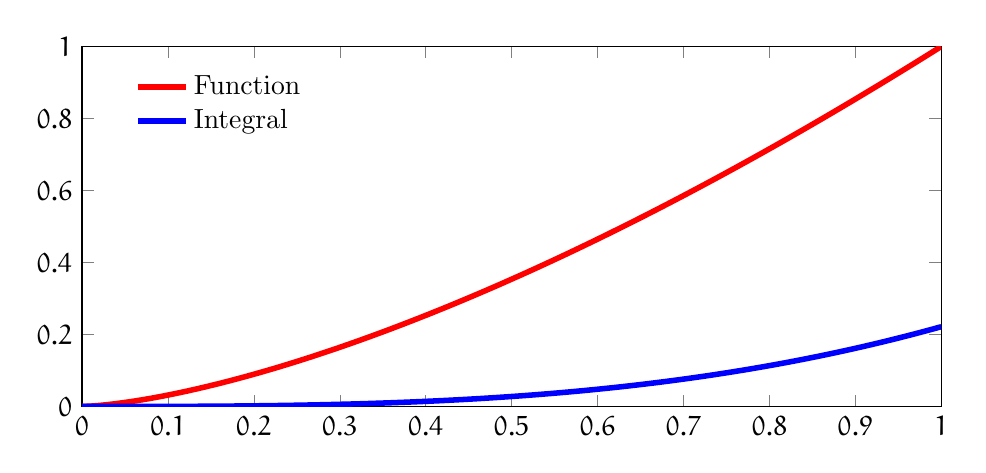
\begin{tikzpicture}

\begin{axis}[%
width=0.9\columnwidth,
height=1.8in,
at={(0.758in,0.481in)},
scale only axis,
xmin=0,
xmax=1,
ymin=0,
ymax=1,
axis background/.style={fill=white},
legend style={at={(0.052,0.728)}, anchor=south west, legend cell align=left, align=left, draw=none, fill=none}
]
\addplot [color=red, line width=2.0pt]
  table[row sep=crcr]{%
0	0\\
0.0101010101010101	0.00101518971238304\\
0.0202020202020202	0.00287139011926748\\
0.0303030303030303	0.005275080483506\\
0.0404040404040404	0.00812151769906434\\
0.0505050505050505	0.0113501660347347\\
0.0606060606060606	0.0149201807247676\\
0.0707070707070707	0.018801576587617\\
0.0808080808080808	0.0229711209541398\\
0.0909090909090909	0.0274101222343421\\
0.101010101010101	0.0321031174830166\\
0.111111111111111	0.037037037037037\\
0.121212121212121	0.042200643868048\\
0.131313131313131	0.0475841413101678\\
0.141414141414141	0.0531788892084089\\
0.151515151515152	0.0589771927395093\\
0.161616161616162	0.0649721415925147\\
0.171717171717172	0.0711574850413269\\
0.181818181818182	0.077527533220222\\
0.191919191919192	0.0840770779311963\\
0.202020202020202	0.0908013282778777\\
0.212121212121212	0.0976958577364506\\
0.222222222222222	0.104756560175785\\
0.232323232323232	0.111979612970155\\
0.242424242424242	0.119361445798141\\
0.252525252525253	0.12689871404788\\
0.262626262626263	0.134588275989434\\
0.272727272727273	0.142427173054662\\
0.282828282828283	0.150412612700936\\
0.292929292929293	0.158541953439015\\
0.303030303030303	0.166812691685812\\
0.313131313131313	0.175222450165657\\
0.323232323232323	0.183768967633119\\
0.333333333333333	0.192450089729875\\
0.343434343434343	0.20126376081961\\
0.353535353535354	0.210208016670401\\
0.363636363636364	0.219280977874737\\
0.373737373737374	0.228480843914229\\
0.383838383838384	0.237805887789995\\
0.393939393939394	0.247254451151243\\
0.404040404040404	0.256824939864133\\
0.414141414141414	0.266515819971046\\
0.424242424242424	0.276325613997122\\
0.434343434343434	0.286252897566592\\
0.444444444444444	0.296296296296296\\
0.454545454545455	0.306454482937837\\
0.464646464646465	0.316726174743368\\
0.474747474747475	0.327110131032995\\
0.484848484848485	0.337605150944384\\
0.494949494949495	0.348210071347384\\
0.505050505050505	0.358923764908435\\
0.515151515151515	0.369745138291201\\
0.525252525252525	0.380673130481342\\
0.535353535353535	0.391706711224629\\
0.545454545454545	0.402844879568725\\
0.555555555555556	0.414086662499961\\
0.565656565656566	0.425431113667271\\
0.575757575757576	0.43687731218628\\
0.585858585858586	0.448424361517156\\
0.595959595959596	0.460071388410507\\
0.606060606060606	0.471817541916075\\
0.616161616161616	0.483661992449529\\
0.626262626262626	0.495603930913032\\
0.636363636363636	0.50764256786566\\
0.646464646464647	0.519777132740118\\
0.656565656565657	0.532006873102455\\
0.666666666666667	0.544331053951817\\
0.676767676767677	0.556748957057473\\
0.686868686868687	0.569259880330615\\
0.696969696969697	0.581863137228624\\
0.707070707070707	0.594558056189662\\
0.717171717171717	0.607343980095642\\
0.727272727272727	0.620220265761776\\
0.737373737373737	0.633186283451024\\
0.747474747474748	0.646241416411904\\
0.757575757575758	0.659385060438249\\
0.767676767676768	0.67261662344957\\
0.777777777777778	0.68593552509082\\
0.787878787878788	0.699341196350408\\
0.797979797979798	0.712833079195415\\
0.808080808080808	0.726410626223022\\
0.818181818181818	0.740073300327238\\
0.828282828282828	0.753820574380079\\
0.838383838383838	0.767651930926394\\
0.848484848484849	0.781566861891604\\
0.858585858585859	0.795564868301656\\
0.868686868686869	0.809645460014542\\
0.878787878787879	0.823808155462778\\
0.888888888888889	0.838052481406278\\
0.898989898989899	0.852377972695084\\
0.909090909090909	0.866784172041448\\
0.919191919191919	0.881270629800814\\
0.929292929292929	0.895836903761244\\
0.939393939393939	0.91048255894087\\
0.94949494949495	0.925207167393004\\
0.95959595959596	0.940010308018511\\
0.96969696969697	0.954891566385127\\
0.97979797979798	0.969850534553367\\
0.98989898989899	0.984886810908746\\
1	1\\
};
\addlegendentry{Function}

\addplot [color=blue, line width=2.0pt]
  table[row sep=crcr]{%
0	0\\
0.0101010101010101	2.2833861661528e-07\\
0.0202020202020202	1.82670893292224e-06\\
0.0303030303030303	6.16514264861256e-06\\
0.0404040404040404	1.46136714633779e-05\\
0.0505050505050505	2.854232707691e-05\\
0.0606060606060606	4.93211411889005e-05\\
0.0707070707070707	7.8320145499041e-05\\
0.0808080808080808	0.000116909371707023\\
0.0909090909090909	0.000166458851512539\\
0.101010101010101	0.00022833861661528\\
0.111111111111111	0.000303918698714938\\
0.121212121212121	0.000394569129511204\\
0.131313131313131	0.00050165994070377\\
0.141414141414141	0.000626561163992328\\
0.151515151515152	0.00077064283107657\\
0.161616161616162	0.000935274973656187\\
0.171717171717172	0.00112182762343087\\
0.181818181818182	0.00133167081210031\\
0.191919191919192	0.0015661745713642\\
0.202020202020202	0.00182670893292224\\
0.212121212121212	0.00211464392847411\\
0.222222222222222	0.0024313495897195\\
0.232323232323232	0.00277819594835811\\
0.242424242424242	0.00315655303608963\\
0.252525252525253	0.00356779088461375\\
0.262626262626263	0.00401327952563016\\
0.272727272727273	0.00449438899083855\\
0.282828282828283	0.00501248931193862\\
0.292929292929293	0.00556895052063006\\
0.303030303030303	0.00616514264861256\\
0.313131313131313	0.00680243572758581\\
0.323232323232323	0.00748219978924949\\
0.333333333333333	0.00820580486530331\\
0.343434343434343	0.00897462098744696\\
0.353535353535354	0.00979001818738013\\
0.363636363636364	0.0106533664968025\\
0.373737373737374	0.0115660359474138\\
0.383838383838384	0.0125293965709136\\
0.393939393939394	0.0135448183990018\\
0.404040404040404	0.0146136714633779\\
0.414141414141414	0.0157373257957417\\
0.424242424242424	0.0169171514277929\\
0.434343434343434	0.0181545183912311\\
0.444444444444444	0.019450796717756\\
0.454545454545455	0.0208073564390674\\
0.464646464646465	0.0222255675868649\\
0.474747474747475	0.0237068001928482\\
0.484848484848485	0.025252424288717\\
0.494949494949495	0.0268638099061711\\
0.505050505050505	0.02854232707691\\
0.515151515151515	0.0302893458326335\\
0.525252525252525	0.0321062362050413\\
0.535353535353535	0.033994368225833\\
0.545454545454545	0.0359551119267084\\
0.555555555555556	0.0379898373393672\\
0.565656565656566	0.040099914495509\\
0.575757575757576	0.0422867134268335\\
0.585858585858586	0.0445516041650405\\
0.595959595959596	0.0468959567418296\\
0.606060606060606	0.0493211411889005\\
0.616161616161616	0.0518285275379528\\
0.626262626262626	0.0544194858206864\\
0.636363636363636	0.0570953860688009\\
0.646464646464647	0.059857598313996\\
0.656565656565657	0.0627074925879713\\
0.666666666666667	0.0656464389224265\\
0.676767676767677	0.0686758073490614\\
0.686868686868687	0.0717969678995757\\
0.696969696969697	0.075011290605669\\
0.707070707070707	0.078320145499041\\
0.717171717171717	0.0817249026113914\\
0.727272727272727	0.08522693197442\\
0.737373737373737	0.0888276036198263\\
0.747474747474748	0.0925282875793102\\
0.757575757575758	0.0963303538845712\\
0.767676767676768	0.100235172567309\\
0.777777777777778	0.104244113659224\\
0.787878787878788	0.108358547192014\\
0.797979797979798	0.112579843197381\\
0.808080808080808	0.116909371707023\\
0.818181818181818	0.121348502752641\\
0.828282828282828	0.125898606365934\\
0.838383838383838	0.130561052578601\\
0.848484848484849	0.135337211422343\\
0.858585858585859	0.140228452928859\\
0.868686868686869	0.145236147129849\\
0.878787878787879	0.150361664057012\\
0.888888888888889	0.155606373742048\\
0.898989898989899	0.160971646216657\\
0.909090909090909	0.166458851512539\\
0.919191919191919	0.172069359661393\\
0.929292929292929	0.177804540694919\\
0.939393939393939	0.183665764644817\\
0.94949494949495	0.189654401542786\\
0.95959595959596	0.195771821420526\\
0.96969696969697	0.202019394309736\\
0.97979797979798	0.208398490242117\\
0.98989898989899	0.214910479249369\\
1	0.22155673136319\\
};
\addlegendentry{Integral}

\end{axis}
\end{tikzpicture}%
\end{column}
\end{columns}
\end{onlyenv}
\end{frame}

\section{Quadratures for Fractional Integrals}

\begin{frame}{Quadratures for Fractional Integrals}
\begin{block}{\faLightbulb[regular]\, Quadrature idea}
Let us assume that $f(t)$  is suitably smooth on an interval $(a,b)$. Let\vspace{-0.5em}
\[
h = \frac{b-a}{N}, \quad t_k = a + kh, \quad \text{ with } k=0,1,2,\ldots,N, \quad N \in \mathbb{N}
\]
\vspace{-0.5em}then we can approximate for $t = t_N$ the fractional integral as\vspace{-0.5em}
\[
\begin{split}
\left. {}_{a}D_{b}^{-\alpha} f(t)\right\rvert_{t = t_N} = & \frac{1}{\Gamma(\alpha)} \int_{a}^{t_N} (t_N - \tau)^{\alpha - 1} f(\tau)\,{\rm d}\tau %\\
= \frac{1}{\Gamma(\alpha)} \sum_{k=0}^{N-1} \int_{t_k}^{t_{k+1}} (t_k - \tau)^{\alpha-1} f(\tau)\,{\rm d}\tau.\vspace{-0.5em}
\end{split}
\]
We approximate $f(x)$ with a polynomial $p(x)$ such that we can compute exactly the involved integrals, this yields quadratures by the usual look\vspace{-0.5em}
\[
\left. {}_{a}D_{b}^{-\alpha} f(t)\right\rvert_{t = t_N}  \approx \sum_{k=0}^{N-1} \omega_k f(t_k).
\]
\end{block}

\end{frame}

\subsection{Piecewise constant approximation}

\begin{frame}{Piecewise constant approximation}
We approximate $f(t)$ on the intervals $[t_k,t_k+1)$, $k=0,\ldots,N-1$, selecting
\[
f(t) \approx p(t) \equiv p(t_k), \quad t \in [t_k,t_k+1), \; k=0,1,\ldots,N-1,
\]
from which we get the formula
\[
\begin{split}
\left. {}_{a}D_{b}^{-\alpha} f(t)\right\rvert_{t = t_N} \approx \only<1>{& \frac{1}{\Gamma(\alpha)} \sum_{k=0}^{N-1} f(t_k) \int_{t_k}^{t_k+1}(t_N - \tau)^{\alpha - 1}\,{\rm d}\tau   
=  \frac{1}{\Gamma(\alpha)} \sum_{k=0}^{N-1} f(t_k) \left[ -\frac{1}{\alpha}(t_N - \tau)^{\alpha} \right]_{t_k}^{t_{k+1}} \\
= & \sum_{k=0}^{N-1} f(t_k) \frac{1}{\alpha \Gamma(\alpha)} \left[ (t_N - t_k)^{\alpha} - (t_N - t_{k+1})^{\alpha} \right] \\
= & \sum_{k=0}^{N-1} f(t_k) \frac{1}{\alpha \Gamma(\alpha)} \left[ ( a + hn - a -kh)^{\alpha} - (a + hn -a -(k+1)h)^{\alpha} \right] \\
= & \sum_{k=0}^{N-1} f(t_k) \frac{h^\alpha}{\Gamma(\alpha+1)} \left[ (n-k)^\alpha - (N-k-1)^\alpha \right] 
= } \sum_{k=0}^{N-1} b_{N-k-1}f(t_k), \only<3->{\qquad b_k = \frac{h^\alpha}{\Gamma(\alpha + 1)} [ (k+1)^\alpha - k^\alpha].}
\end{split}
\]
\only<2>{where we have defined
\[b_k = \frac{h^\alpha}{\Gamma(\alpha + 1)} [ (k+1)^\alpha - k^\alpha], \qquad 0 \leq k \leq N-1.\]}
\only<3>{Analogously we get the case in which we select the \textbf{right approximation}
\[
f(t) \approx p(t) \equiv p(t_{k+1}), \quad t \in [t_k,t_k+1), \; k=0,1,\ldots,N-1,
\]
and, more generally, for the \textbf{weighted formula} in which we select
\[
f(t) \approx p(t) \equiv \lambda p(t_{k}) + (1-\lambda)p(t_{k+1}), \quad t \in [t_k,t_k+1), \; k=0,1,\ldots,N-1, \; \lambda \in [0,1].
\]
}\only<4>{The general \textbf{weighted formula} is then given by
\[
\left. {}_{a}D_{b}^{-\alpha} f(t)\right\rvert_{t = t_N} \approx \sum_{k=0}^{N-1} b_{N-k-1} \left[ \lambda p(t_{k}) + (1-\lambda)p(t_{k+1}) \right], \quad \lambda \in [0,1].
\]
}
\end{frame}

\begin{frame}{Implementation}
This is a simple procedure to implement
\inputminted[bgcolor=bg,fontsize=\footnotesize,breaklines]{matlab}{constfracint.m}
\end{frame}

\begin{frame}[fragile]{Implementation - II}
And we can \textbf{test the results} using the fractional integral we have computed by hand
\definecolor{bg}{rgb}{0.95,0.95,0.95}
\begin{minted}[bgcolor=bg,fontsize=\footnotesize,breaklines]{matlab}
f     = @(t,mu) t.^mu;
Itrue = @(alpha,mu,t) gamma(mu+1)*t.^(alpha+mu)/ gamma(alpha+mu+1);
mu    = 1;
alpha = 1.5;

N = 100;
lambda = 1;
I = constfracint(@(t) f(t,mu),0,1,alpha,N,1);
fprintf('Relative error is: %e\n',abs(I-Itrue(alpha,mu,1))./abs(Itrue(alpha,mu,1)));
\end{minted}
That returns us
\definecolor{bg}{rgb}{0.95,0.95,0.95}
\begin{minted}[bgcolor=bg,fontsize=\footnotesize,breaklines]{bash}
Relative error is: 1.246939e-02
\end{minted}
But \alert{what about convergence}?
\end{frame}

\begin{frame}{Convergence}
\begin{columns}
\begin{column}{0.5\columnwidth}
\begin{block}{Fractional Newton-Cotes formula}
Lef $f(t)$ be approximated by a polynomial $p_{k,r}(t)$ of degree $r$ on the
grid points $\{t_k = t_0^{(k)},\ldots,t_{r}^{(k)} = t_{k+1}\}$. Then the error
estimate for an $f \in \mathcal{C}^{r+1}([a,b])$ on each sub-interval $[t_k,t_{k+1}]$ is given by
\[ f(t)-p_{k,r}(t) = \frac{f^{(r+1)}(\tau_k)}{(r+1)!} \prod_{j=0}^{r} (t - t_j^{(k)}), \]
for $r \in \mathbb{N}$, $t,\tau_k \in [t_k,t_{k+1}]$, i.e., the formula is of order $O(h^{r+1})$.
\end{block}

\end{column}
\begin{column}{0.35\columnwidth}
\scriptsize\centering
% This file was created by matlab2tikz.
%
%The latest updates can be retrieved from
%  http://www.mathworks.com/matlabcentral/fileexchange/22022-matlab2tikz-matlab2tikz
%where you can also make suggestions and rate matlab2tikz.
%
\definecolor{mycolor1}{rgb}{0.00000,0.44700,0.74100}%
\definecolor{mycolor2}{rgb}{0.85000,0.32500,0.09800}%
\definecolor{mycolor3}{rgb}{0.92900,0.69400,0.12500}%
%
\begin{tikzpicture}

\begin{axis}[%
width=0.8\columnwidth,
height=1.5in,
at={(0.772in,0.481in)},
scale only axis,
xmode=log,
xmin=10,
xmax=100000,
xminorticks=true,
xlabel style={font=\color{white!15!black}},
%xlabel={N},
ymode=log,
ymin=1e-12,
ymax=1,
yminorticks=true,
ylabel style={font=\color{white!15!black}},
title={Relative Error},
axis background/.style={fill=white},
legend style={at={(0.03,0.03)}, anchor=south west, legend cell align=left, align=left, draw=none, fill=none}
]
\addplot [color=mycolor1, line width=2.0pt, mark=o, mark options={solid, mycolor1}]
  table[row sep=crcr]{%
10	0.122076348118973\\
100	0.0124693871170266\\
1000	0.00124968951478086\\
10000	0.000124996881371206\\
100000	1.24999687702464e-05\\
};
\addlegendentry{$\lambda\text{ = 1}$}

\addplot [color=mycolor2, dashed, line width=2.0pt, mark=x, mark options={solid, mycolor2}]
  table[row sep=crcr]{%
10	0.127923651881027\\
100	0.0125306128829735\\
1000	0.00125031048521914\\
10000	0.000125003118628905\\
100000	1.25000312301153e-05\\
};
\addlegendentry{$\lambda\text{ = 0}$}

\addplot [color=mycolor3, dashdotted, line width=2.0pt, mark=square, mark options={solid, mycolor3}]
  table[row sep=crcr]{%
10	0.00292365188102693\\
100	3.06128829734672e-05\\
1000	3.10485219139851e-07\\
10000	3.11862875745755e-09\\
100000	3.12300266581296e-11\\
};
\addlegendentry{$\lambda\text{ = 0.5}$}

\end{axis}
\end{tikzpicture}%
\begin{tabular}{cccc}
\toprule
$N$/$\lambda$ & $0$ & $1$ & $\nicefrac{1}{2}$ \\
\midrule
1e+01 & 1.3e-01 & 1.2e-01 & 2.9e-03 \\
1e+02 & 1.3e-02 & 1.2e-02 & 3.1e-05 \\
1e+03 & 1.3e-03 & 1.2e-03 & 3.1e-07 \\
1e+04 & 1.3e-04 & 1.2e-04 & 3.1e-09 \\
1e+05 & 1.3e-05 & 1.2e-05 & 3.1e-11 \\
\bottomrule
\end{tabular}
\end{column}
\end{columns}
\end{frame}

\begin{frame}{Convergence}
\textbf{Proof.}\only<1>{The interpolating polynomial can be expressed in the \textbf{Lagrange basis}
\[
p_{k,r}(t) = \sum_{i=0}^{r} l_{k,i}(t) f(t_i^{(k)}), \quad l_{k,i}(t) = \prod_{\substack{j=0\\j\neq i}}^r \frac{t - t_j^{(k)}}{t_i^{(k)}-t_j^{(k)}}, \quad 0 \leq i \leq r, \; t \in [t_{k},t_{k+1}].
\]
}Then the \alert{fractional Newton-Coates} formula si given by
\[
\left. {}_{a}D_{b}^{-\alpha} f(t)\right\rvert_{t = t_N} \approx \left. {}_{a}D_{b}^{-\alpha} p_{k,r}(t)\right\rvert_{t = t_N} = \sum_{k = 0}^{N-1} \sum_{i=0}^{r} C_{i,N}^{(k)} f(t_i^{(k)}),
\]
\only<1>{for
\[
C_{i,N}^{(k)} = \frac{1}{\Gamma(\alpha)} \int_{t_k}^{t_{k+1}}(t_N - \tau)^{\alpha-1} l_{k,i}(\tau)\,\textrm{d}\tau.
\]}
\only<2->{from which we obtain the error estimate as
\[
\begin{split}
\left| {}_{a}D_{b}^{-\alpha} f(t) - {}_{a}D_{b}^{-\alpha} p_{k,r}(t) \right| \only<2-3>{\leq & \frac{1}{\Gamma(\alpha)} \sum_{k=0}^{N-1} \int_{t_k}^{t_{k+1}} (t_N - \tau)^{\alpha-1} \left| f(\tau) - p_{k,r}(\tau) \right|\,\textrm{d}\tau \\
\leq & \max_{t \in [a,t_N]} \frac{|f^{(r+1)}(t)|}{ (r+1)! \Gamma(\alpha)} \sum_{k=0}^{N-1} \int_{t_k}^{t_{k+1}} (t_N - \tau)^{\alpha-1} \prod_{j=0}^{r} |\tau - t_j^{(k)}|\,\textrm{d}\tau \\
\leq & \max_{t \in [a,t_N]} \left| f^{(r+1)}(t) \right| \frac{h^{r+1}}{(r+1)! \Gamma(\alpha\only<3>{+1})} \only<2>{\sum_{k=0}^{N-1} \int_{t_k}^{t_{k+1}} (t_N - \tau)^{\alpha-1}\,\textrm{d}\tau}\only<3>{(t_N - t_0)^{\alpha}}.}\only<4->{\in O(h^{r+1}).} 
\end{split}
\]
}
\begin{onlyenv}<4>
\begin{exampleblock}{Remark}
The error estimate does not coincide completely with the classical one for Newton-Coates formulas, this is due to the nonsymmetry of the integral kernel $(t_N' - t)^{\alpha-1}$.
\end{exampleblock}
\end{onlyenv}
\end{frame}

\begin{frame}{Suggested exercises, and some extensions}
\definecolor{danger}{HTML}{f0ad4e}
\begin{enumerate}[(i)]
\item Rewrite (and implement) the fractional weighted constant approximation for the \emph{other-sided} Riemann-Liuoville fractional integral,
\item Denote with $t_{k + \nicefrac{1}{2}} = \nicefrac{t_{k} + t_{k+1}}{2}$ on each sub-interval $[t_k,t_{k+1}]$, approximate $f(t)$ with a \emph{piecewise quadratic polynomial}, derive and implement the fractional Simpson's formula -- \textcolor{danger}{\faExclamationTriangle} The closed form of the coefficients for this case is cumbersome\ldots
\end{enumerate}

\begin{block}{Extensions}
By mimicking the usual procedure for deriving collocation/spectral type quadrature formulas, we could approximate $f(t)$ by using, e.g., Jacobi polynomials to obtain the related quadrature formulas (when you have obtained formulas for Jacobi, then \emph{Chebyshev} and \emph{Legendre} follow with relative ``ease'').
\end{block}

\end{frame}

\section{Riemann--Liouville Fractional Derivatives}

\begin{frame}{Riemann--Liouville Fractional Derivatives}
Now that we've gotten a little bit of familiarity with Riemann--Liouville integral operators, we can finally \textbf{introduce the corresponding differential operators}.

\begin{block}{\faLightbulb[regular]\,The key idea \only<2>{ \alert{now we go from integers to real numbers!} }}
Let $f$ be a function having a continuous $n$th derivative on the interval $[a,b]$, and let $m \in \mathbb{N}$ be such that $m > n$, then
\[
 \frac{d^n}{d t^n} f(t) = \frac{1}{(m-n-1)!} \frac{d^m}{d t^m} \int_{a}^{t} (t-\tau)^{m-n-1} f(\tau)\,{\rm d}\tau = \frac{d^m}{d t^m}  I_a^{m-n} f,
\]
simply by employing the \alert{Fundamental Theorem of (Classical) Calculus}
\[
f = \frac{d^{m-n}}{d t^{m-n}} I_a^{m-n}f,
\]
and applying the operator $\frac{d^n}{d t^n}$ to both side of it.
\end{block}
\end{frame}

\begin{frame}{Riemann--Liouville Fractional Derivatives}
\definecolor{danger}{HTML}{f0ad4e}
Substitute the integer $n$ with a real positive number $\alpha$ and select an $m \in \mathbb{N}$ s.t. $m > \alpha$.

\begin{block}{RL Derivative}
Let $\alpha \in \mathbb{R}_+$ and $m = \lceil \alpha \rceil$, we define the Riemann-Liouville operator ${}_\text{RL}D_a^\alpha$ as
\[
{}_\text{RL}D_a^\alpha f(t) \triangleq \frac{d^m}{d t^m} I_a^{m-\alpha} f(t),
\]
and we set ${}_\text{RL}D_a^0$ to the identity operator.
\end{block}

\begin{itemize}
	\item[{\textcolor{danger}{\faExclamationTriangle}}] The right-hand side of our definition remains valid, \alert{\textbf{but}} now the resulting operator \alert{depends on the choice of the point $a$}.
	\item<2>[{\faQuestionCircle}] for what functions $f$ does this definition make sense?
\end{itemize}

\end{frame}

\begin{frame}{Riemann--Liouville Fractional Derivatives Existence}

\begin{block}{The $\mathbb{A}^n$ functions}
We call $\mathbb{A}^n[a,b]$, or simply $\mathbb{A}^n$ when the interval is
clear from the context, the space of function with an \textbf{absolutely continuous}
$(n-1)$st derivative, i.e., the functions $f$ for which there exists almost
everywhere a (generalized) $n$th derivative function $g \in \mathbb{L}^1[a,b]$ for which holds
\[
f^{(n-1)}(t) = f^{(n-1)}(a) + \int_{a}^{t} g(\tau)\,{\rm d}\tau.
\]
\end{block}

\begin{description}
	\item[Remind:] For a compact interval:
	\begin{center}
		    continuously differentiable $\subseteq$ Lipschitz continuous $\subseteq$ absolutely continuous $\subseteq$ bounded variation $\subseteq$ differentiable almost everywhere
	\end{center}
	\item[Example:] $f(t) = \sqrt[3]{t}$ is absolutely continuous on any bounded interval $I$ \textbf{but} not Lipschitz continuous on any interval $I$ such that $0 \in I$.
\end{description}

\end{frame}

\begin{frame}{Riemann--Liouville Fractional Derivatives Existence}
\begin{alertblock}{Theorem (Existence)}
Lef $f \in \mathbb{A}^1[a,b]$, and $0 < \alpha < 1$. Then ${}_\text{RL}D_a^\alpha f(t)$ exists almost everywhere in $[a,b]$. Moreover, ${}_\text{RL}D_a^\alpha f(t) \in \mathbb{L}^p$ for $1 \leq p < \alpha^{-1}$ and
\[
{}_\text{RL}D_a^\alpha f(t) = \frac{1}{\Gamma(1-\alpha)} \left( \frac{f(a)}{(t-a)^\alpha} + \int_{a}^{t} f'(\tau)(t-\tau)\,{\rm d}\tau \right).
\]
\end{alertblock}

\textbf{Proof.} We use directly the two definitions\only<3>{, and apply again \emph{Fubini's Theorem}}\only<4>{, and finally Leibniz rule for the derivative of integral functions,}
\[
\begin{split}
{}_\text{RL}D_a^\alpha f(t) \only<1>{
= & \frac{1}{\Gamma(1-\alpha)} \frac{d}{d t} \int_{a}^{t} f(\tau)(t-\tau)^{-\alpha}\,{\rm d}\tau \\
= & \frac{1}{\Gamma(1-\alpha)} \frac{d}{d t} \int_{a}^{t} \left( f(a) + \int_{a}^{\tau} f'(s)\,{\rm d}s \right)(t-\tau)^{-\alpha}\,{\rm d}\tau \\
}
\only<2>{
= & \frac{1}{\Gamma(1-\alpha)} \frac{d}{d t} \int_{a}^{t} \left( f(a) + \int_{a}^{\tau} f'(s)\,{\rm d}s \right)(t-\tau)^{-\alpha}\,{\rm d}\tau \\
= & \frac{1}{\Gamma(1-\alpha)} \frac{d}{d t} \left( f(a)\int_{a}^{t} \frac{{\rm d}t}{(x-t)^\alpha} + \int_{a}^{t}\int_{a}^{\tau} f'(s)(t-\tau)^{-\alpha}\,{\rm d}s\,{\rm d}\tau\right) \\
}
\only<3>{
= & \frac{1}{\Gamma(1-\alpha)} \frac{d}{d t} \left( f(a)\int_{a}^{t} \frac{{\rm d}t}{(x-t)^\alpha} + \int_{a}^{\tau}\int_{a}^{t} f'(s)(t-\tau)^{-\alpha}\,{\rm d}s\,{\rm d}\tau\right) \\
= & \frac{1}{\Gamma(1-\alpha)} \left( \frac{f(a)}{(t-a)^{\alpha}} + \frac{d}{dt} \int_{a}^{\tau} \int_{a}^{t} f'(s)(t-\tau)^{-\alpha}\,{\rm d}s\,{\rm d}\tau \right) \\
\text{(Fubini) }= &  \frac{1}{\Gamma(1-\alpha)} \left( \frac{f(a)}{(t-a)^\alpha} + \frac{d}{dt} \int_{a}^{t} f'(s) \frac{(t-s)^{1-\alpha}}{1-\alpha}\,{\rm d}s \right),
}
\only<4>{
= & \frac{1}{\Gamma(1-\alpha)} \left( \frac{f(a)}{(t-a)^\alpha} + \frac{d}{dt} \int_{a}^{t} f'(s) \frac{(t-s)^{1-\alpha}}{1-\alpha}\,{\rm d}s \right), \\
\text{(Leibniz) }= & \frac{1}{\Gamma(1-\alpha)} \left( \frac{f(a)}{(t-a)^\alpha} + \int_{a}^{t} f'(\tau)(t-\tau)\,{\rm d}\tau \right).
}
\end{split}
\]
\end{frame}

\begin{frame}{Computing our first RL derivatives}
To keep things simple we can compute, first of all, the fractional derivative of order $\alpha \in (0,1)$ of the \textcolor{blue}{\textbf{constant function}} $f(t) = 1$ in $[0,t]$:

\begin{columns}
\begin{column}{0.6\columnwidth}
We simply apply the previous representation theorem, and thus:
\[
\begin{split}
{}_\text{RL}D_{[0,1]}^\alpha f(t) = & \frac{1}{\Gamma(1-\alpha)} \left( \frac{f(0)}{(t-0)^\alpha} + \int_{0}^{t} f'(\tau)(t-\tau)\,{\rm d}\tau \right) = \\
= & \frac{1}{\Gamma(1-\alpha)} \frac{1}{(t-0)^\alpha} = \frac{t^{-\alpha}}{\Gamma(1-\alpha)}
\end{split}
\]
\end{column}
\begin{column}{0.3\columnwidth}
% This file was created by matlab2tikz.
%
%The latest updates can be retrieved from
%  http://www.mathworks.com/matlabcentral/fileexchange/22022-matlab2tikz-matlab2tikz
%where you can also make suggestions and rate matlab2tikz.
%
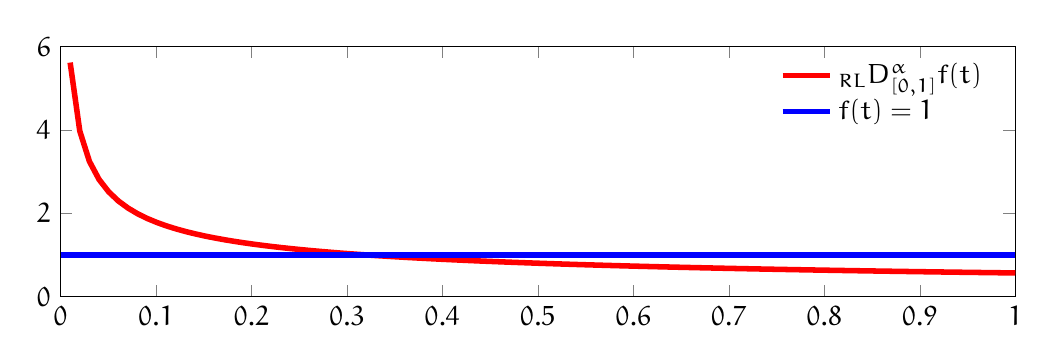
\begin{tikzpicture}

\begin{axis}[%
width=\columnwidth,
height=1.25in,
at={(0.758in,0.481in)},
scale only axis,
unbounded coords=jump,
xmin=0,
xmax=1,
ymin=0,
ymax=6,
axis background/.style={fill=white},
legend style={legend cell align=left, align=left, draw=none, fill=none}
]
\addplot [color=red, line width=2.0pt]
  table[row sep=crcr]{%
0	inf\\
0.0101010101010101	5.61361547776433\\
0.0202020202020202	3.96942557130092\\
0.0303030303030303	3.24102240721429\\
0.0404040404040404	2.80680773888217\\
0.0505050505050505	2.5104851615652\\
0.0606060606060606	2.29174892211877\\
0.0707070707070707	2.12174721572964\\
0.0808080808080808	1.98471278565046\\
0.0909090909090909	1.87120515925478\\
0.101010101010101	1.77518108181096\\
0.111111111111111	1.69256875064327\\
0.121212121212121	1.62051120360714\\
0.131313131313131	1.55693680352443\\
0.141414141414141	1.5003018442061\\
0.151515151515152	1.44942928382623\\
0.161616161616162	1.40340386944108\\
0.171717171717172	1.36150173861321\\
0.181818181818182	1.32314185710031\\
0.191919191919192	1.28785171449845\\
0.202020202020202	1.2552425807826\\
0.212121212121212	1.22499132615384\\
0.222222222222222	1.1968268412043\\
0.232323232323232	1.17051974208776\\
0.242424242424242	1.14587446105939\\
0.252525252525253	1.12272309555287\\
0.262626262626263	1.10092057165103\\
0.272727272727273	1.08034080240476\\
0.282828282828283	1.06087360786482\\
0.292929292929293	1.04242222453938\\
0.303030303030303	1.02490127544389\\
0.313131313131313	1.00823510334604\\
0.323232323232323	0.99235639282523\\
0.333333333333333	0.97720502380584\\
0.343434343434343	0.962727111970672\\
0.353535353535354	0.948874201088476\\
0.363636363636364	0.935602579627389\\
0.373737373737374	0.922872699666136\\
0.383838383838384	0.910648680484574\\
0.393939393939394	0.898897882626065\\
0.404040404040404	0.88759054090548\\
0.414141414141414	0.876699446958561\\
0.424242424242424	0.866199673618086\\
0.434343434343434	0.856068334756042\\
0.444444444444444	0.846284375321634\\
0.454545454545455	0.8368283871884\\
0.464646464646465	0.827682447142981\\
0.474747474747475	0.818829973936544\\
0.484848484848485	0.810255601803572\\
0.494949494949495	0.801945068252047\\
0.505050505050505	0.793885114260184\\
0.515151515151515	0.786063395290478\\
0.525252525252525	0.778468401762215\\
0.535353535353535	0.771089387816798\\
0.545454545454545	0.763916307372923\\
0.555555555555556	0.756939756606048\\
0.565656565656566	0.750150922103052\\
0.575757575757576	0.743541534042\\
0.585858585858586	0.737103823831362\\
0.595959595959596	0.730830485715236\\
0.606060606060606	0.724714641913115\\
0.616161616161616	0.718749810915958\\
0.626262626262626	0.712929878606305\\
0.636363636363636	0.707249071909879\\
0.646464646464647	0.701701934720542\\
0.656565656565657	0.696283305870372\\
0.666666666666667	0.690988298942671\\
0.676767676767677	0.685812283748423\\
0.686868686868687	0.680750869306603\\
0.696969696969697	0.675799888186137\\
0.707070707070707	0.670955382082629\\
0.717171717171717	0.666213588516383\\
0.727272727272727	0.661570928550153\\
0.737373737373737	0.657023995435492\\
0.747474747474748	0.652569544105861\\
0.757575757575758	0.648204481442857\\
0.767676767676768	0.643925857249224\\
0.777777777777778	0.639730855868769\\
0.787878787878788	0.63561678839912\\
0.797979797979798	0.631581085448371\\
0.808080808080808	0.6276212903913\\
0.818181818181818	0.623735053084926\\
0.828282828282828	0.619920124006894\\
0.838383838383838	0.616174348783474\\
0.848484848484849	0.612495663076922\\
0.858585858585859	0.608882087804655\\
0.868686868686869	0.605331724665073\\
0.878787878787879	0.60184275194706\\
0.888888888888889	0.598413420602149\\
0.898989898989899	0.595042050560108\\
0.909090909090909	0.59172702727032\\
0.919191919191919	0.588466798452782\\
0.929292929292929	0.585259871043878\\
0.939393939393939	0.582104808323267\\
0.94949494949495	0.579000227209334\\
0.95959595959596	0.575944795711636\\
0.96969696969697	0.572937230529693\\
0.97979797979798	0.569976294788274\\
0.98989898989899	0.567060795900131\\
1	0.564189583547756\\
};
\addlegendentry{${}_\text{RL}D_{[0,1]}^\alpha f(t)$}

\addplot [color=blue, line width=2.0pt]
  table[row sep=crcr]{%
0	1\\
0.0101010101010101	1\\
0.0202020202020202	1\\
0.0303030303030303	1\\
0.0404040404040404	1\\
0.0505050505050505	1\\
0.0606060606060606	1\\
0.0707070707070707	1\\
0.0808080808080808	1\\
0.0909090909090909	1\\
0.101010101010101	1\\
0.111111111111111	1\\
0.121212121212121	1\\
0.131313131313131	1\\
0.141414141414141	1\\
0.151515151515152	1\\
0.161616161616162	1\\
0.171717171717172	1\\
0.181818181818182	1\\
0.191919191919192	1\\
0.202020202020202	1\\
0.212121212121212	1\\
0.222222222222222	1\\
0.232323232323232	1\\
0.242424242424242	1\\
0.252525252525253	1\\
0.262626262626263	1\\
0.272727272727273	1\\
0.282828282828283	1\\
0.292929292929293	1\\
0.303030303030303	1\\
0.313131313131313	1\\
0.323232323232323	1\\
0.333333333333333	1\\
0.343434343434343	1\\
0.353535353535354	1\\
0.363636363636364	1\\
0.373737373737374	1\\
0.383838383838384	1\\
0.393939393939394	1\\
0.404040404040404	1\\
0.414141414141414	1\\
0.424242424242424	1\\
0.434343434343434	1\\
0.444444444444444	1\\
0.454545454545455	1\\
0.464646464646465	1\\
0.474747474747475	1\\
0.484848484848485	1\\
0.494949494949495	1\\
0.505050505050505	1\\
0.515151515151515	1\\
0.525252525252525	1\\
0.535353535353535	1\\
0.545454545454545	1\\
0.555555555555556	1\\
0.565656565656566	1\\
0.575757575757576	1\\
0.585858585858586	1\\
0.595959595959596	1\\
0.606060606060606	1\\
0.616161616161616	1\\
0.626262626262626	1\\
0.636363636363636	1\\
0.646464646464647	1\\
0.656565656565657	1\\
0.666666666666667	1\\
0.676767676767677	1\\
0.686868686868687	1\\
0.696969696969697	1\\
0.707070707070707	1\\
0.717171717171717	1\\
0.727272727272727	1\\
0.737373737373737	1\\
0.747474747474748	1\\
0.757575757575758	1\\
0.767676767676768	1\\
0.777777777777778	1\\
0.787878787878788	1\\
0.797979797979798	1\\
0.808080808080808	1\\
0.818181818181818	1\\
0.828282828282828	1\\
0.838383838383838	1\\
0.848484848484849	1\\
0.858585858585859	1\\
0.868686868686869	1\\
0.878787878787879	1\\
0.888888888888889	1\\
0.898989898989899	1\\
0.909090909090909	1\\
0.919191919191919	1\\
0.929292929292929	1\\
0.939393939393939	1\\
0.94949494949495	1\\
0.95959595959596	1\\
0.96969696969697	1\\
0.97979797979798	1\\
0.98989898989899	1\\
1	1\\
};
\addlegendentry{$f(t) = 1$}

\end{axis}
\end{tikzpicture}%
\end{column}
\end{columns}
\vfill

\onslide<2>{\centering \alert{The RL derivative of a constant is not zero!}}

\end{frame}

\begin{frame}{Computing our first RL derivatives}
Let $f(t) = (t-a)^\beta$ for some $\beta > -1$ and compute its RL derivative of order $\alpha > 0$ on an interval $[a,b]$.

First we compute the \textbf{fractional integral} part of the definition:
\[
\begin{split} 
I_{[a,t]}^\alpha f(t) = \only<1>{& \frac{1}{\Gamma(\alpha)} \int_{a}^{t} (\tau - a)^\beta (t - \tau)^{\alpha - 1}\,\textrm{d}\tau = \\
= & \frac{1}{\Gamma(\alpha)} \int_{0}^{t-a} s^\beta (t-a-s)^{\alpha-1} \,\textrm{d}s = \textcolor{gray}{\leftarrow \left( \int_{0}^{x} s^{\beta - 1}(x-s)^{\alpha - 1} \textrm{d}s = \frac{\Gamma(\alpha)\Gamma(\beta)}{\Gamma(\alpha+\beta)}x^{\alpha+\beta-1}  \right)} \\
= &} \frac{\Gamma(\beta + 1)}{\Gamma(\alpha + \beta + 1)} (t - a)^{\alpha+\beta},
\end{split}
\]
\only<2>{Then we just have to compute the derivative with the correct indexes
\[
\begin{split}
{}_\text{RL}D_{[0,1]}^\alpha f(t) = & \frac{d^{\lceil \alpha \rceil}}{d t^{{\lceil \alpha \rceil}} } I_{[a,t]}^{{\lceil \alpha \rceil} - \alpha} f(t) = \frac{\Gamma(\beta + 1)}{\Gamma(\lceil \alpha \rceil - \alpha + \beta + 1) } \left.\frac{d^{\lceil \alpha \rceil}}{d t^{{\lceil \alpha \rceil}} } (\cdot - a)^{\lceil \alpha \rceil - \alpha + \beta}\right|_t,
\end{split}
\]
now, if $\alpha - \beta \in \mathbb{N}$ the right-hand side vanishes ($\lceil\alpha\rceil$-derivative of a polynomial of lower degree), if $\alpha - \beta \not\in \mathbb{N}$, we find
\[
\begin{split}
{}_\text{RL}D_{[0,1]}^\alpha f(t) = \frac{\Gamma(\beta + 1)}{\Gamma(\beta + 1 - \alpha)} (t-a)^{\beta - \alpha}.
\end{split}
\]
}
 
\end{frame}

\begin{frame}{Summary and anticipations}
\definecolor{success}{HTML}{4a934a}
\definecolor{todo}{HTML}{0099cc}

We did
\begin{itemize}
	\item[\textcolor{success}{\faCheckCircle}] Definition and properties of Riemann--Liouville Integrals,
	\item[\textcolor{success}{\faCheckCircle}] Some examples of Fractional Newton-Cotes formulas for RL integral computations,
	\item[\textcolor{success}{\faCheckCircle}] Definition and  existence of Riemann--Liouville Derivatives,
	\item[\textcolor{success}{\faCheckCircle}] A couple of by-hand computations of RL derivatives of simple functions.
\end{itemize}

Next up
\begin{itemize}
	\item[\textcolor{todo}{\faClipboardList}] Properties and interactions between Riemann--Liouville Integrals and Derivatives,
	\item[\textcolor{todo}{\faClipboardList}] The Caputo fractional derivative,
	\item[\textcolor{todo}{\faClipboardList}] An introduction to Fractional Differential Equations.
\end{itemize}

\end{frame}

\appendix

\section*{Bibliography}
{\unnumbered
\begin{frame}[allowframebreaks]{Bibliography}
\small
\printbibliography

\end{frame}
}
\end{document}

